\chapter{Aplicación y Estimación de Parámetros}


Espero que el siguiente capítulo nos lleve de la mano para generar un modelo con la siguientes propiedades:

\begin{enumerate}
    \item Cada arista en el grafo se le considera una variable aleatoria
    \item Una hipótesis de dependencia es propuesta definiendo relaciones sobre las variables de nuestro grafo
    \item La hipótesis de dependencia implica una forma particular al modelo gracias al teorema de Hammersley–Clifford, (Besag, 1974). 
    \item Simplificación de parámetros implica una forma particular al modelo
    \item Estimación y interpretación de los parámetros del modelo.
\end{enumerate}

\section{Estado espacios generales}

Brevemente si $(X , B)$ es un espacio medible y tenemos un $K(x, dy)$ kernel de Markov con una medida de probabilidad $K(x,\cdot )$. Si iteramos por el Kernel de tal forma que $(x, A) = Z$. Entonces tenemos una distribución estacionaría $\pi(dx)$ que satisface que $\pi(A) = ZK(x,A)(dx)$.

%Aqui este parrafo esta requetemal

\subsection{Motivación}
  \begin{theorem}{De representación en general (Hewwit y Savage, 1955)}
 \\ Si $(X_{1}, X_{2}, X_{3},...)$ es una sucesión de variables aleatorias intercambiables, entonces
 \begin{enumerate}
     \item Existen una función $g(x_{1},x_{2},x_{3},...,x_{n})$ y un modelo probabilístico $p(x\vert \theta),x\in X$ con $$\theta= lim_{n \to \infty} g(x_{1},x_{2},x_{3},...,x_{n}), \; \theta \in   \Theta$$
     \item Existe una función de densidad $p(\theta)$ tal que $$\mathcal{P}(\theta)=\int_{\Theta}\prod^{n}_{i=1} p(x_{i}\vert \theta)p(\theta)d\theta$$
     \end{enumerate}
 \end{theorem}
La segunda parte del Teorema en esencia confirma que para cualesquiera $(X_{1},...,X_{n})$ intercambiables éstas deben de ser interpretadas como una muestra aleatoria de un modelo de probabilidades y nos dice cómo calcularlo. Este modelo depende de un parámetro $\theta$, afortunadamente el teorema nos garantiza su existencia como una función límite de las observaciones y que además tiene un modelo de probabilidad asociado ($p(\theta)$). \\ 

Estos teoremas son teoremas de la teoría de la probabilidad y no dependen en lo absoluto de a qué escuela de la estadística pertenezcas. \\ A partir de estos resultados el procedimiento para realizar inferencia estadística paramétrica debe de ser el siguiente \\
Supongamos que tenemos un conjunto de observaciones $(x_{1},x_{2},...,x_{n})$ y nos interesa estimar un parámetro $\phi$ relacionado a ellas. El proceso se descompone en tres fases: \begin{enumerate}

    \item Especificación del modelo \\
    Se define un modelo $P(x\vert \theta)$ de forma que las observaciones sean variables aleatorias condicionalmente independientes, a partir de esto obtenemos que $P(x_{1},x_{2},x_{3},...,x_{n}\vert \theta)=\prod^{n}_{i=1} p(x_{i}\vert \theta)$ donde $\theta =\lim_{x \to \infty} f(x_{1},x_{2},x_{3},...,x_{n})$ para alguna función $f$.\\
    \item Especificación de la distribución inicial\\
    Cualquier información que tenemos sobre $\theta$ debe de ser descrita por $p(\theta)$, esta mide la incertidumbre que tenemos sobre el valor $\theta$ y debe de contener toda la información con la que contemos.\\
   
    \item Determinación de la distribución final de la magnitud de interés
    \\Se aplica el teorema de Bayes y el teorema de la probabilidad total y obtenemos, las siguientes dos ecuaciones:
    \begin{equation}
        p(\theta\vert x_{1},x_{2},...,x_{n}) \propto \prod^{n}_{i=1} p(x_{i}\vert \theta)p(\theta)
    \end{equation}
    \begin{equation}
        p(\phi\vert x_{1},x_{2},...,x_{n})=\int_{\Theta} p(\phi\vert \theta)p(\theta\vert x_{1},x_{2},...,x_{n})d\theta
    \end{equation}

\end{enumerate}

\section{Metropolis-Hastings y estimación de parámetros con muestreo de Gibbs}

Sea $\mathcal{X}$ un espacio finito y $\pi(x)$ una probabilidad sobre $\mathcal{X}$ especificada hasta una constante normalizadora desconocida. Sea $J(x,y)$ una matriz de Markov sobre X con $J(x,y) > 0$ si y sólo si $J(y,x) > 0$. En un principio J no está relacionada con $\pi$. El algoritmo de Metropolis Hastings actualiza J a una nueva matriz de Markov $K(x,y)$ con distribución estacionaria $\pi$. 

\subsection{Comentarios}
Una característica importante del modelo que puede ayudar en la interpretación es que si, por ejemplo, un grafo tiene muchas dos-estrellas presentes, entonces algunas van a formar triángulos de forma aleatoria. Sin embargo, si existiese un efecto triángulo significativo en nuestro \textit{ERGM}, y este efecto está por encima del efecto de dos-estrellas entonces podemos inferir que el nivel de triangulación no ocurre simplemente por procesos aleatorios. Podemos concluir que la triangulación es un efecto importante en este grafo independiente de otros efectos.

El algoritmo de \textit{Metropolis-Hastings} empieza con la definición de una cadena de Markov que tiene una distribución $\pi(\cdot)$ estacionaria.

Cuando los términos dependientes de díadas están en el modelo, los algoritmos computacionales en \textit{ERGM} usan Monte Carlo vía cadenas de Markov (MCMC), con una muestra de Metropolis-Hastings, para estimar los parámetros. Este enfoque básicamente funciona de la siguiente manera.
\subsection{Muestreo de Gibbs}

El muestreo de Gibbs especifica que todos los elementos $Y_{ij}$ son aleatoriamente actualizados. Si, en el paso t del muestro el elemento $Y_{ij}$ es el que está siendo actualizado entonces un nuevo valor es generado de acuerdo a la probabilidad condicional sobre todos los elementos de tal forma que:

\begin{equation}
    \mathrm{P}_{\theta}\left\{Y_{i j}^{(t+1)}=a | Y^{(t)}=y^{(t)}\right\}\\
    
= \mathrm{P}_{\theta}\left\{Y_{i j}=a | Y_{h k}=y_{h k}^{(t)} \text { para todo }(h, k) \neq(i, j)\right\}
\end{equation}

donde $a=0,1$. En este paso todos los elementos no están siendo actualizados entonces $Y_{ij}^{t+1} = Y_{hk}^{t}$ para todo $(h,k) \neq (i,j)$. El teorema general de \cite{StochasticRelaxation} implica que la distribución de $Y_t$ converge cuando $t \to \infty$ para la distribución de probabilidad de los grafos aleatorios exponenciales. Para una matriz de adyacencia y cualquiera obtenida donde se define el elemento $y_{ij}^{(ij1)} = 1$ y $y_{ij}^{(ij0)} = 0$ y dejando todos los elementos como están en y entonces la distribución condicional está definida como

\begin{equation*}
    \operatorname{logit}\left(\mathrm{P}_{\theta}\left\{Y_{i j}=1 | Y_{h k}=y_{h k} \text { para todo }(h, k) \neq(i, j)\right\}\right) \\
    
\quad=\theta^{\prime}\left(u\left(y^{(i j 1)}\right)-u\left(y^{(i j 0)}\right)\right)
\end{equation*}

en otras palabras esto significa que la distribución condicional está definida por un modelo regresión logística en donde las estadísticas suficientes están dadas por las diferencias entre los valores de $u(y)$ obtenido cuando se actualizan los elementos $y_{ij} = 1$ o $y_{ij} = 0$ y dejando todos los otros elementos igual.

%El muestreo de Gibbs puede experimentar problemas de convergencia severos pues el modelo puede no simular los efectos correctamente o la estimación del parámetro puede resultar en una explosión de diadas de donde resultan distribuciones bimodales que consisten de estados de alta y baja densidad en donde los estados se definen como un subconjunto del espacio muestral. Adicionalmente existen una variedad de estados no estrictamente limitados a los bimodales.

\subsection{Metrópolis Hastings}

El algoritmo de Metrópolis y otros como éste fueron inventados para estudiar propiedades de equilibrio como promedios de ensamblaje, evolución en el tiempo, ambientes de baja temperatura, interacción de componentes en un sistema grande y homogéneo como las moléculas de gas.


\subsection{Implementación}

Es necesario comenzar con un vector inicial de valores de parámetros; el valor predeterminado es usar las estimaciones de máxima pseudo verosimilitud \cite{Besag1974}, usando el algoritmo de estimación de regresión logística. Empezamos al elegir una díada al azar y se lanza una moneda, ponderada por el modelo, para decidir si habrá un empate. Se hace esto para 1024 pasos (el intervalo MCMC predeterminado para el periodo de \textit{burn in}). Tomamos la red en el último paso y calculamos las estadísticas de la red (las del modelo). Hacemos esto 1024 veces (el tamaño de muestra MCMC predeterminado). Calculamos el promedio de cada estadística en la muestra y la comparamos con la estadística observada. Entonces actualizamos las estimaciones de los parámetros según sea necesario. Repetimos hasta que el proceso converja; es decir que la diferencia entre el promedio de la muestra MCMC y la diferencia entre la estadística observada y la del promedio de la muestra generada es suficientemente pequeña.

%Poner lo que es permisible para el modelo y los observado

\begin{algorithm}[H]
\SetLine
\KwData{Y}
\KwResult{Muestreo de Gibbs}
inicializamos un $x^{0}\thicksim g(x)$\; \\
\While{iteración $i = 1,2,\ldots,$}{
$x_{1}^{(i)} \sim p\left(X_{1}=x_{1} | X_{2}=x_{2}^{(i-1)}, X_{3}=x_{3}^{(i-1)}, \ldots, X_{D}=x_{D}^{(i-1)}\right)$\\
$x_{2}^{(1)} \sim p\left(X_{2}=x_{2} | X_{1}=x_{1}^{(i)}, X_{3}=x_{3}^{(i-1)}, \ldots, X_{D}=x_{D}^{(i-1)}\right)$\\
$\dot{\vdots}$\\
${x_{D}^{(i)}} \sim p\left(X_{D}=x_{D} | X_{1}=x_{1}^{(i)}, X_{2}=x_{2}^{(i)}, \ldots, X_{D}=x_{D-1}^{(i)}\right)$\\

}
\caption{Muestreo de Gibbs}
\end{algorithm}

\subsection{Consideraciones adicionales}

Cada término en un \textit{ERGM} debe tener un algoritmo asociado para calcular su valor para su red. El paquete \textit{ergm} en statnet de R incluye alrededor de 150 algoritmos de computación. Exploramos algunos de estos términos en esta tesis, y se proporcionan enlaces a más información en el apéndice.

\subsection{Problema a resolver}

Una vez que ya introducimos distintos tipos de estadísticas, hablamos sobre los niveles de dependencia markoviana y de nuestro poderosísimo arsenal de algortimos para el cálculo de los parámetros de nuestro modelo logístico ajustado vale la pena recordar que el modelo general de dependencia de los ERGMs tiene la forma de

\begin{equation}
    p(y=Y)=\frac{1}{\psi(Z)} \exp \left\{\sum_{A \in Z} \theta_{A} \cdot z_{A}(Y)\right\}
\end{equation}

donde A es para indicar el \textit{clique} que pertenece a Z nuestro espacio muestral de nuestro grafo que incluye todos los posibles \textit{cliques}. El valor $\theta$ tendrá valores positivos cuando la probabilidad de observar el grafo $y$ se incrementa. 

Existen formas de condicionamiento de este modelo general de tal forma que las aristas sean producto de los atributos nodales o los que nos interesan en este caso que son los modelos con dinámicas orientadas a aristas o de dependencia diádica que funcionan mejor cuando se trata de un grafo no dirigido como el que vamos a analizar en el caso empírico posterior.

Para resolver los problemas de degeneración de los ERGM cuando estimamos el modelo a partir de las estadísticas de cambio que causan efectos de cascada y nos llevan a los grafos completos o los grafos vacíos. Así que lo que hacemos es que generamos una simulación en donde el grafo se construye añadiendo arista por arista hasta que se llegue a la máxima verosimilitud. Esta función de probabilidad es en sí una función de las estadísticas de cambio y se ven impactados por el cambio en log odds para una diada adicional, o cualquier efecto. Es decir, si una arista adicional significa que se hacen dos nuevas 2 estrellas, entonces la log probabilidad de observar esa arista incrementa por dos multiplicado por el parámetro de las dos-estrellas. 


En efecto un modelo de grafos aleatorios se define como estable si pequeños cambios en el espacio de parámetros resultan en cambios pequeños en la estructura probabilística del modelo \cite{Snidjers2010}. Los parámetros del modelo controlan la creación y configuración de los \textit{cliques} que son esperados en el grafo. Como existen efectos cascada entre la interacción de las estadísticas elegidas es entonces que éstas ejemplifican la transición de fase para ciertos valores del parámetro en donde el número esperado de, por ejemplo el de triángulos triángulos, incrementa exponencialmente. Los grafos más grandes son más susceptibles a estos efectos de modalidad cuando el número de nodos incrementa pues estos pueden contener un mayor numero de subestructuras.

Para resolver este problema utilizamos la solución de \cite{snijders_markov_2002} en donde agregamos variables basadas en el concepto de dependencia condicional parcial. Agregamos un peso a la distribución del modelo dándole alto peso a la baja densidad mientras que se reducen los pesos conforme el grado de la variable incrementa. Es decir que

\begin{equation*}
    u_{\alpha}^{(d)}=\sum_{k=0}^{n-1} e^{-\alpha k} d_{k}(y)
\end{equation*}

donde $d_k(y)$ es el numero de nodos con grado k y $\alpha$ es el parámetro de los pesos. Esto es la medida geométrica de distribución de grados. En caso particular tenemos que el modelo se ve de forma 

\begin{equation*}
    u_{\lambda}^{s}=S_{2}-\frac{S_{3}}{\lambda}+\frac{S_{4}}{\lambda^{2}}-\ldots+(-1)^{n-2} \cdot \frac{S_{n-1}}{\lambda^{n-3}}=\sum_{k=2}^{n-1}(-1)^{k} \cdot \frac{S_{k}}{\lambda^{k-2}}
\end{equation*}

donde $S_k$ es el numero de estrellas de grado $k$ y $\lambda$ es el parámetro. Este es el método de las estrellas de k-estrellas alternadas. La diferencia entre la distribución geométrica de $k$ grados y la de $k$ estrellas corresponde a la de los los signos alternados. Un valor grande de 3-estrellas está balanceado por el valor negativo de las 4 estrellas por el cambio de signo. La adición de los pesos asegura que los cambios en la estadísticas sean pequeñas y de hecho las estadísticas de cambio en particular son escritas como

\begin{equation*}
    z_{i j}=-\left(1-e^{-\alpha}\right)\left(e^{-\alpha y_{i+}}+e^{-\alpha y_{j+}}\right)
\end{equation*}

donde $\Tilde{y}_{i+}$ es la densidad cuando la arista entre $i$ y $j$ es agregada. El valor de la estadística de cambio es reducido por el factor $-(1-e^{-\alpha})$. Este factor asegura que estas estadísticas de cambio no tomen valores altos y resulten en una distribución acotada. 

Ahora sólo falta estimar el modelo.

\subsection{Ajuste del modelo}

El algoritmo Metropolis-Hasting elige una variable del grafo aleatoriamente y cambia su estado. La probabilidad del nuevo grafo es calculada si y solamente si la probabilidad de esta nueva realización del grafo es más probable que la anterior. La regla se decisión se basa en la razón de Hastings para maximizar la verosimilitud sin tener que tener una constante normalizadora $\psi(\theta)$

\begin{equation*}
    min \left\{1, \dfrac{p_{\theta(x^{*})}}{p_{\theta}(x^{m-1})}\right\}.
\end{equation*}

Los pasos que toma el algoritmo son pequeños para no sobrepasar el óptimo global. Aunque el algoritmo de Metropolis-Hastings es lento, es sumamente preciso en su estimación. 

Entonces para los modelos ERGM estimamos utilizando la función de máxima verosimilitud. Empezando de la forma canónica del ERGM definimos nuestra función de verosimilitud como antes

\begin{equation}
    p(y=Y)=\frac{1}{\psi(Z)} \exp \left\{\sum_{A \in Z} \theta_{A} \cdot z_{A}(Y)\right\}.
\end{equation}

Sin embargo, aquí desconocemos el valor de la constante normalizadora que no puede ser obtenida computacionalmente. Afortunadamente podemos mejorar nuestra estimación de la logverosimilitud a través del uso de métodos de aproximación log normal. Como desconocemos el valor de la constante entonces podemos trabajar alrededor de la dificultad computacional y proveer parámetros iniciales $(\theta_0)$. Así puede podemos escribir nuestra log verosimilitud para el modelo canónico \cite{RProject}

\begin{equation*}
    L(\theta)-L\left(\theta_{0}\right)=\left(\theta-\theta_{0}\right)^{T} V(G)-\log E_{\theta_{0}}\left[\exp \left(\theta-\theta_{0}\right)^{T} V(g)\right].
\end{equation*}

Geyer \cite{StochasticRelaxation} nos dice que al maximizar esta ecuación generando una muestra de la distribución de los grafos generados a partir de $\theta_0$ sólo se comportan bien cuando $\theta$ está cercano a $\theta_0$. Para encontrar una solución a esta problema del parámetro inicial al algoritmo al suponer que la función de máxima verosimilitud no es el valor observado de los parámetros sino algún punto entre los valores promedio de la parametrización y un valor observado $\omega$ entonces definimos los pasos del algoritmo solución: 

\begin{equation*}
    \hat{\omega}_{t}=\gamma_{t} \cdot v(G)+\left(1-\gamma_{t}\right) \bar{\omega}
\end{equation*}

donde $w_t$ representa el valor de la estimación en espacio parametral promedio. Idealmente quisiéramos que $\bar{\omega}$ fuera igual a 1 para que así el valor esperado de los parámetros fuese el valor observado.

\begin{enumerate}
    \item Iniciamos eligiendo valores para el vector $\theta_0$
    \item Usamos MCMC para simular de la gráfica con la función de probabilidad el vector $\theta_0$
    \item Calculamos la media de la muestra
    \item Definimos una pseudo observación que es una combinación convexa  entre la media de la muestra y el valor observado
    \item Reemplazamos la observación por la pseudo observación y repetimos los pasos 2 a 5
\end{enumerate}

Para esta tesis usaremos el algoritmo de \textit{Robbins-Monro} utilizados por  \cite{Snidjers2002} para estimar modelos de ERGM. El método estima

\begin{equation*}
    E\left\{Z_{\theta}\right\}=0
\end{equation*}

donde $Z_{\theta}$ es el vector de parámetros que satisfacen que $u(Y) = u_0$ donde $u_0$ es el valor observado de las estadísticas. Así reescribimos la ecuación como una ecuación de momentos en donde el algoritmo da los valores iniciales que son iguales al promedio de los promedios de los parámetros. Para hacer los pasos del algoritmo entonces definimos 

\begin{equation*}
    \theta^{t+1}=\theta^{t}-a_{t} \cdot D^{-1}\left(z\left(x^{m}\right)-z\left(x_{o b s}\right)\right)
\end{equation*}

donde $D$ es la matriz de covarianza cuyos elementos de la diagonal de la matriz son utilizados como la matriz de escala y $a$ define la convergencia y está puesto de tal forma que $a_t = \dfrac{a_{t-1}}{2}$. Suponemos que la función de máxima verosimilitud es la correcta cuando $z(x^m) - z(x_{obs})$ es cercano a cero.

\subsection{Bondad de ajuste y degeneración del modelo}

Existen dos cosas que hacer una vez que hayamos generado el modelo. Primero probaremos nuestras cadenas MCMC, después haremos pruebas gráficas de bondad de ajuste con los valores de las estadísticas para un número grande de grafos simulados con el modelo ajustado. Para hacer esto en las ERGM se consideran 3 conjuntos de estadísticas: el grado de ciertos atributos del nodo, las diadas compartidas y la distribución de la distancia geodésica.


Consideremos un simple modelo dependiente de las diadas. Cuando éste converge correctamente debemos de ver que la desviación del valor de la estadística muestreada de cada grafo y el valor observado de la distribución de las desviaciones de la muestra estén variando aleatoriamente alrededor del valor observado en cada paso (para garantizar que nuestra cadena se esté mezclando correctamente). Los valores muestreados deberían de mostrar poca correlación y que la diferencia entre el valor observado y los valores simulados de la estadística se vean normal y centrados alrededor de 0. 

La distribución de grado para un grafo consiste de los valores $\dfrac{D_0}{n}
,...,\dfrac{D_{n - 1}}{n}$ que son iguales a la proporción de nodos que comparten aristas con exactamente $k$ otros nodos. Los valores de diada o pareja compartida consisten de los valores $\dfrac{EP_0}{E},...,\dfrac{EP_{n-2}}{E}$ que son el número total de aristas y $EP_k$ es el número de aristas cuya punta comparte aristas con exactamente k otros nodos. Finalmente, la distancia geodésica consiste de la frecuencia relativa de los posibles valores de la distancia geodésica entre cualesquiera dos nodos donde la distancia geodésica es la longitud del camino más corto que une a esos dos nodos (o infinito si ese camino no existe). Por ejemplo, dos nodos están a distancia 1 si están conectados y además existen $n \choose 2$ posibles pares de nodos, el primer valor de la distancia geodésica es igual a $\dfrac{E}{{n \choose 2}} $. El último valor, la fracción con diadas con distancia geodésicas infinitas se dice que es inalcanzable.

El grado de un nodo es el número de vecinos que tiene donde un vecino es un nodo que comparte con ese una arista. Definimos entonces $D_k(y)$ que sea el número de nodos que tiene el grafo y con grado $k$. Nótese que las estadísticas $D_k(y)$ cumplen la condición que $\sum_{i=0)}^{n-1}D_i(y) = n$. Una formulación de las estadísticas de k estrellas $S_1(y),\ldots,S_{n-1}(y)$, en donde $S_k(y)$ es el número de k estrellas en el grafo también definimos para 1 estrella de tal forma que

\begin{equation*}
    S_{k}(\mathbf{y})=\sum_{i=k}^{n-1}\left(\begin{array}{l}i \\ k\end{array}\right) D_{i}(\mathbf{y}), \quad 2 \leq k \leq n-1 
\end{equation*}
\begin{equation*}
    S_{1}(\mathbf{y})=\frac{1}{2} \sum_{i=1}^{n-1} i D_{i}(\mathbf{y})
\end{equation*}

Estas estadísticas contienen mucha información relevante de nuestro grafo. Denotamos el número de k-triángulos y diadas en el grafo. $T_k(y)$ y $P_k(y)$. Las estadísticas $D_i$ son las estadísticas de grado

\begin{equation*}
    T_{k}(\mathbf{y})=\sum_{i=k}^{n-2}\left(\begin{array}{l}i \\ k\end{array}\right) E P_{i}(\mathbf{y}), \quad 2 \leq k \leq n-2
\end{equation*}
y
\begin{equation*}
    P_{k}(\mathbf{y})=\sum_{i=k}^{n-2}\left(\begin{array}{l}i \\ k\end{array}\right) D P_{i}(\mathbf{y}), \quad 1 \leq k \leq n-2, k \neq 2.
\end{equation*}

Con este fin definimos las estadísticas

\begin{equation*}
    u(\mathbf{y} ; \tau)=e^{\tau} \sum_{i=1}^{n-2}\left\{1-\left(1-e^{-\tau}\right)^{i}\right\} D_{i}(\mathbf{y})
\end{equation*}

\begin{equation*}
    v(\mathbf{y} ; \tau)=e^{\tau} \sum_{i=1}^{n-2}\left(1-\left(1-e^{-\tau}\right)^{i}\right\} E P_{i}(\boldsymbol{y})
\end{equation*}

\begin{equation}
    w(\mathbf{y} ; \tau)=e^{\tau} \sum_{i=1}^{n-2}\left\{1-\left(1-e^{-\tau}\right)^{i}\right\} D P_{i}(\mathbf{y})
\end{equation}

donde en cada caso de las estadísticas tenemos que $\tau$ es un parámetro adicional. Estas estadísticas son las ya mencionadas  grado geométrico, las diadas de parejas compartidas y las estadísticas de las diadas de parejas compartidas.

Aunque estas definiciones de nuestras nuevas estadísticas $u,v$ y $w$ podrán parecer magia negra en realidad coinciden con las estrellas alternantes, alternando k-triángulos y alternando las estadísticas de k parejas de \cite{snijders_markov_2002} 


\begin{equation*}
    u(\mathbf{y} ; \tau)=2 S_{1}(\mathbf{y})-\frac{S_{2}(\mathbf{y})}{\left(e^{\tau}\right)^{1}}+\cdots+(-1)^{n} \frac{S_{n-1}(\mathbf{y})}{\left(e^{\tau}\right)^{n-2}}

\end{equation*}

\begin{equation*}
    v(\mathbf{y} ; \tau)=3 T_{1}(\mathbf{y})-\frac{T_{2}(\mathbf{y})}{\left(e^{\tau}\right)^{1}}+\cdots+(-1)^{n-3} \frac{T_{n-2}(\mathbf{y})}{\left(e^{\tau}\right)^{n-3}}

\end{equation*}


\begin{equation*}
    w(\mathbf{y} ; \tau)=P_{1}(\mathbf{y})-\frac{2 P_{2}(\mathbf{y})}{\left(e^{\tau}\right)^{1}}+\cdots+(-1)^{n-3} \frac{P_{n-2}(\mathbf{y})}{\left(e^{\tau}\right)^{n-3}.}
\end{equation*}


De hecho esta última no es idéntica a la estadística de Snidjers \cite{GoodOfFitSocialNetwork} pero se dice podría decir que es de cierta forma equivalente desde un punto de vista de construcción del modelo. 

Los modelos de grafos pueden ser como generativos cuando son ellos mismos quienes representan el proceso que gobierna los patrones esféricos de prevalencia de las aristas desde una perspectiva local: la perspectiva de los nodos que están involucrados en comportamiento local representan cada una de ellas un término en el modelo \textit{ERGM}. El proceso local generativo entonces agrega hasta producir ciertas características en las propiedades del grafo aunque estas propiedades esféricas no se encuentren explícitamente en el modelo.

Una prueba de un modelo que se ajusta a los datos es uno que reproduce las propiedades esféricas que no están en el modelo. Hacemos esto al elegir una estadística que no está en el modelo y comparamos el valor de la estadística que no incluimos en nuestro modelo para ajustar nuestro modelo utilizando los principios de bondad de ajuste que se han declarado.

Podremos ver cuando un modelo no es una buena representación de un grafo observado, los grafos generados en nuestras cadenas de MCMC pueden aparecer lo suficiente lejos del grafo observado que el proceso de estimación se verá afectado, en el peor de los casos, que los grafos simulados sean tan diferentes que el algoritmo falle completamente. Cuando esto sucede significa que no se pudo llevar a cabo la estimación. El modelo que hubiese especificado de cualquier grafo que hubieses simulado entonces no pudo haber producido el grafo observado. Algunos modelos, ahora que sabemos, casi nunca producen nada interesante con alguna densidad, puro ruido, aquí es cuando hemos experimentado la degeneración del modelo.

Afortunado es que aún en en estos casos donde no podremos ser capaces de estimar coeficientes que funcionen entonces aún podemos usar la función de bondad de ajuste para identificar cómo es que el modelo simulado se desvía de los datos observados. De hecho, aún podremos utilizar los diagnósticos del muestreo de MCMC para observar que está fallando dentro del algoritmo de solución, además de que nos brinda con la experiencia y la intuición de los comportamientos de los términos de \textit{ERGM} nos pueda dar ideas para mejorar la especificación del modelo. Aún cuando fallamos tenemos que seguir iterando. La paquetería de statnet de R afortunadamente detiene el algoritmo después de 3 iteraciones para no explotar nuestra memoria y podemos observar el trabajo hecho hasta ese momento para inspeccionar en nuestra artillería\footnote{algoritmo} pesada\footnote{de muestreo}.

La degeneración es un indicador de un modelo mal especificado como nos dice \cite{Snidjers2010} no es una característica de todos los \textit{ERGM} pero si está asociado con algunos términos diádicos en particular los modelos de Markov reducidos homogéneos (Utilizando 2 estrellas y los términos de triángulo).

\section{Matrimonio Florentino}

Empezamos con un caso muy simple de una multitud de datos que vienen disponibles en el la paquetería de grafos \textit{igraph} de R: El Matrimonio Florentino. Este es un conjunto de datos hecho por Padgett (1944) que describe los matrimonios que existen entre las familias florentinas más importantes. Los datos vienen en una matriz de adyacencia simétrica. Este conjunto de datos contiene información sobre 16 nodos y 20 aristas entre las familias. También existe información de los nodos como la riqueza de cada familia.


Comenzamos con la implementación del modelo Bernoulli o Erd\H{o}s Rényi que incluye únicamente un parámetro sobre las aristas del grafo.

\begin{figure}[t]
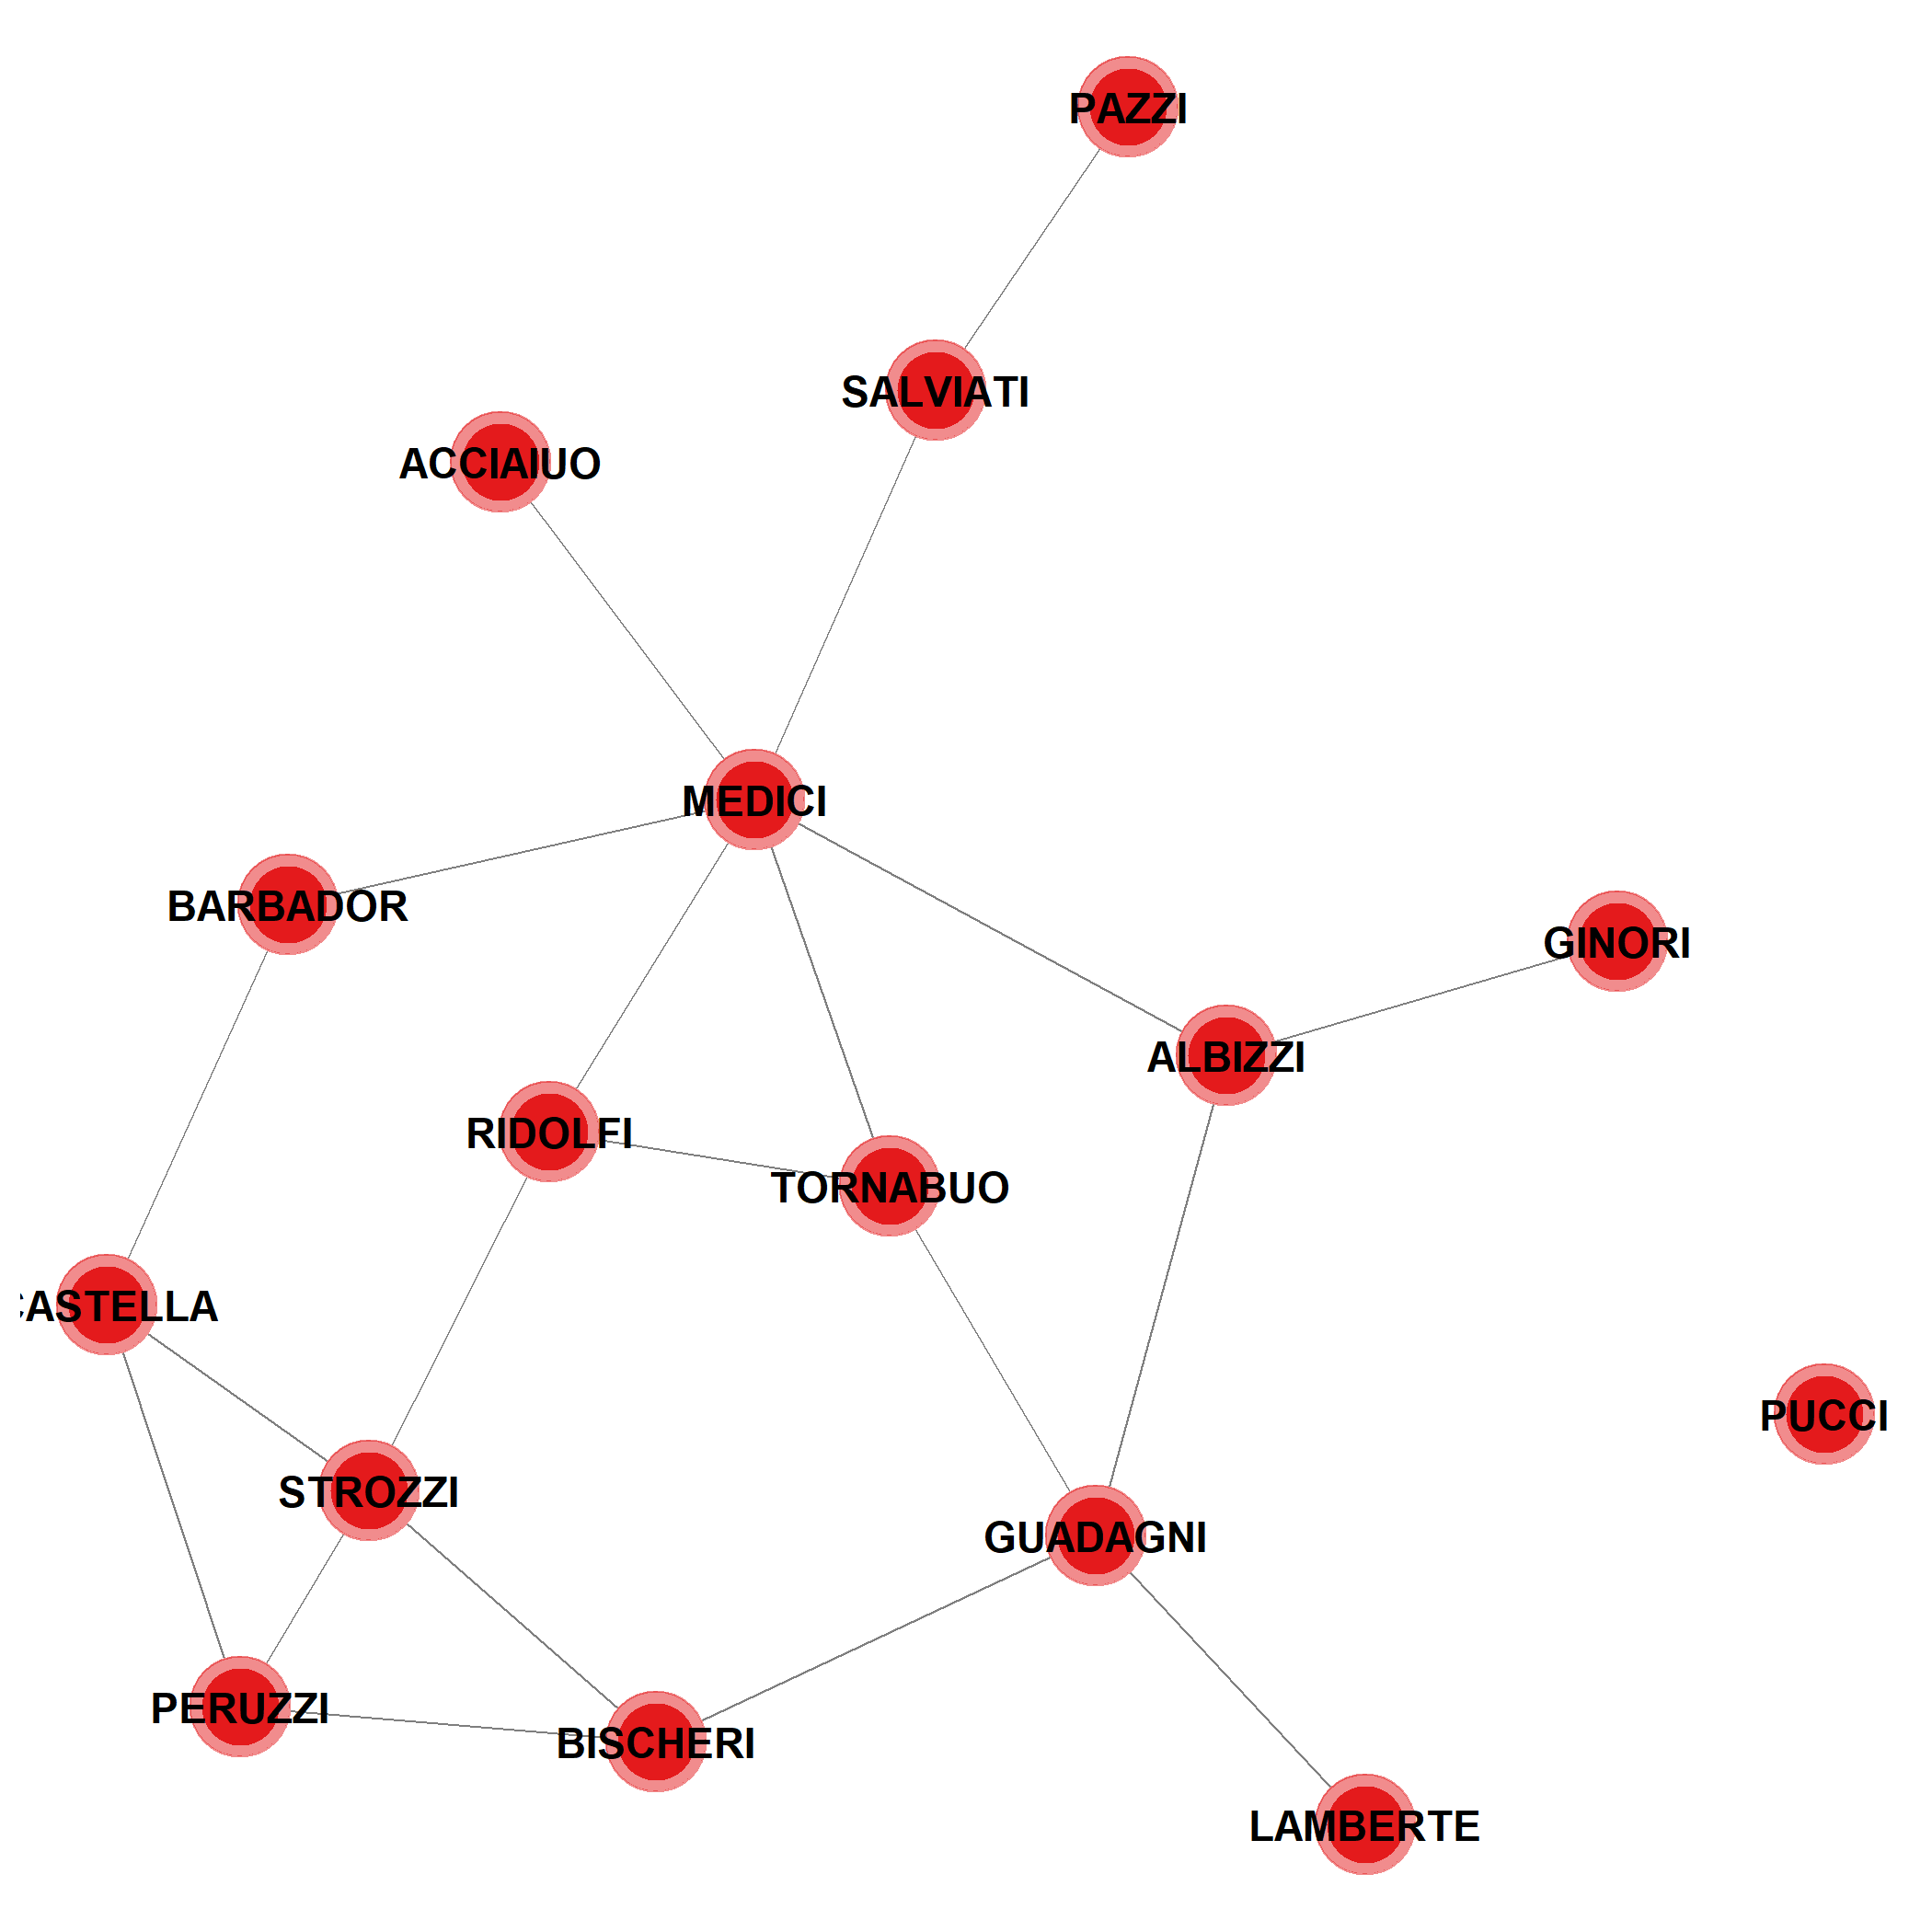
\includegraphics[width=.75\textwidth]{Tesis/Figures/Florentine.png}
\caption{El Matrimonio Florentino}
\centering
\end{figure}

Empezamos con el modelo de tal forma que expresemos nuestro modelo.

\begin{equation*}
    \textit{Florentino} \sim \textit{Numero.de.Aristas}
\end{equation*}

\begin{equation*}
    \log \left( \exp \left( \theta ^ { \prime } g ( y ) \right) \right) = \theta _ { 1 }  \sum _ { i , j > i \in \mathcal{N} } y _ { i j }.    
\end{equation*}

El modelo nos entrega entonces los estimadores de los parámetros de tal forma que nuestro estimador de $\theta_1=-1.6094$  y nos da un valor p significativo. ¿Cómo interpretamos esto?

\begin{equation*}
\begin{split}
    \operatorname{logit}(p(y))&=\theta \times \delta(g(y))\\
    &=-1.6094 \times \Delta Numero\hspace{} de\hspace{} aristas \\
    &=-1.6094 \times 1
\end{split}
\end{equation*}


Para cada arista, agregar cualquier arista a nuestro grafo siempre incrementa nuestro número de aristas por 1. La probabilidad correspondiente es obtenida sacando el $logit$ inverso de $\theta$:

\begin{equation*}
\begin{split}
    &= \exp (-1.61) /(1+\exp (-1.61))\\
    &= 0.1665886
\end{split}
\end{equation*}

Interpretamos el modelo de tal forma que esta probabilidad corresponde a la densidad que observamos en nuestro grafo de $20$ aristas y un posible de $120$ aristas que pudiese haber con los 16 nodos. Es decir que la probabilidad de una arista es $20/120=.16\bar{6}$.

Avanzamos en nuestro proceso de modelaje añadiendo el término de triángulos para considerar un elemento de conglomerado:

\begin{equation*}
    \textit{Florentino} \sim \textit{Numero.de.Aristas} + \textit{Numero.de.Triángulos}
\end{equation*}

\begin{equation*}
    \log \left( \exp \left( \theta ^ { \prime } g ( y ) \right) \right) = \theta _ { 1 } \times \sum _ { i , j > i \in \mathcal{N} } y _ { i j }  + \theta_2    \times \sum _ { i j k }  y _ { i j } y _ { j k } y _ { k i } 
\end{equation*}

Este modelo nos brinda entonces que los valores estimados de los parámetros de las aristas son $\theta_1 = -1.6694$ y $\theta_2 = 0.1539$. Es decir que las log-\textit{odds} para que una arista no termine por crear ningún triángulo el condicional log-\textit{odds} es entonces de $-1.67$. Para que entonces forme un triángulo los log-\textit{odds} se convierte en $-1.67+ .0.1539 = -1.516$, entonces que se hagan dos triángulos tenemos que $-1.67+2 \times 0.1539 = -1.34$. Las correspondientes probabilidades entonces son $0.1584, 0.1801, 0.2039$ respectivamente.

Para este caso normalmente se puede utilizar el atributo de riqueza de cada familia con la covarianza entre cada familia como parte de nuestro modelo. Sin embargo, nos vamos a enfocar en las dinámicas orientadas a aristas ya que es lo que haremos más adelante. Además, también veremos el caso de los pesos geométricos con k estrellas y su correspondiente análisis.

Inspeccionado la última ronda de simulación antes del cálculo de las las estimaciones del parámetro tenemos acceso a la traza y la densidad de cada estadística.

\begin{figure}[t]
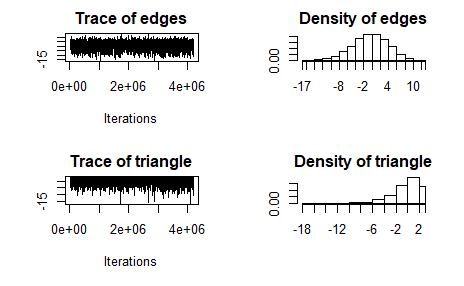
\includegraphics[width=1\textwidth]{Tesis/Figures/mcmcflorentine.jpg}
\caption{Diagnóstico de las cadenas de Markov}
\centering
\end{figure}

De aquí podemos observar que nuestro modelo se comporta de forma adecuada pues nuestras distribuciones están centradas y la traza es aleatoria. Aún así esto no nos garantiza que estos procesos locales estén capturando toda la información y que sean capaces de generar grafos que tengan las mismas propiedades globales.

Entonces simulamos 100 grafos con los parámetros estimados y comparamos en la siguiente tabla:

\begin{center}
 \begin{tabular}{||c c c||} 
 \hline
 Num & Aristas & Triángulo \\ [.5ex] 
 \hline\hline
 Obs & 20.00 & 3.0 \\ 
 \hline
 Media Simulada & 20.47 & 3.3  \\
 \hline
\end{tabular}
\end{center}

Vemos que nuestra estimación se encuentra bien ajustada para las aristas y que tiene un error del 10\% en esta serie de simulaciones.

\begin{figure}[h]
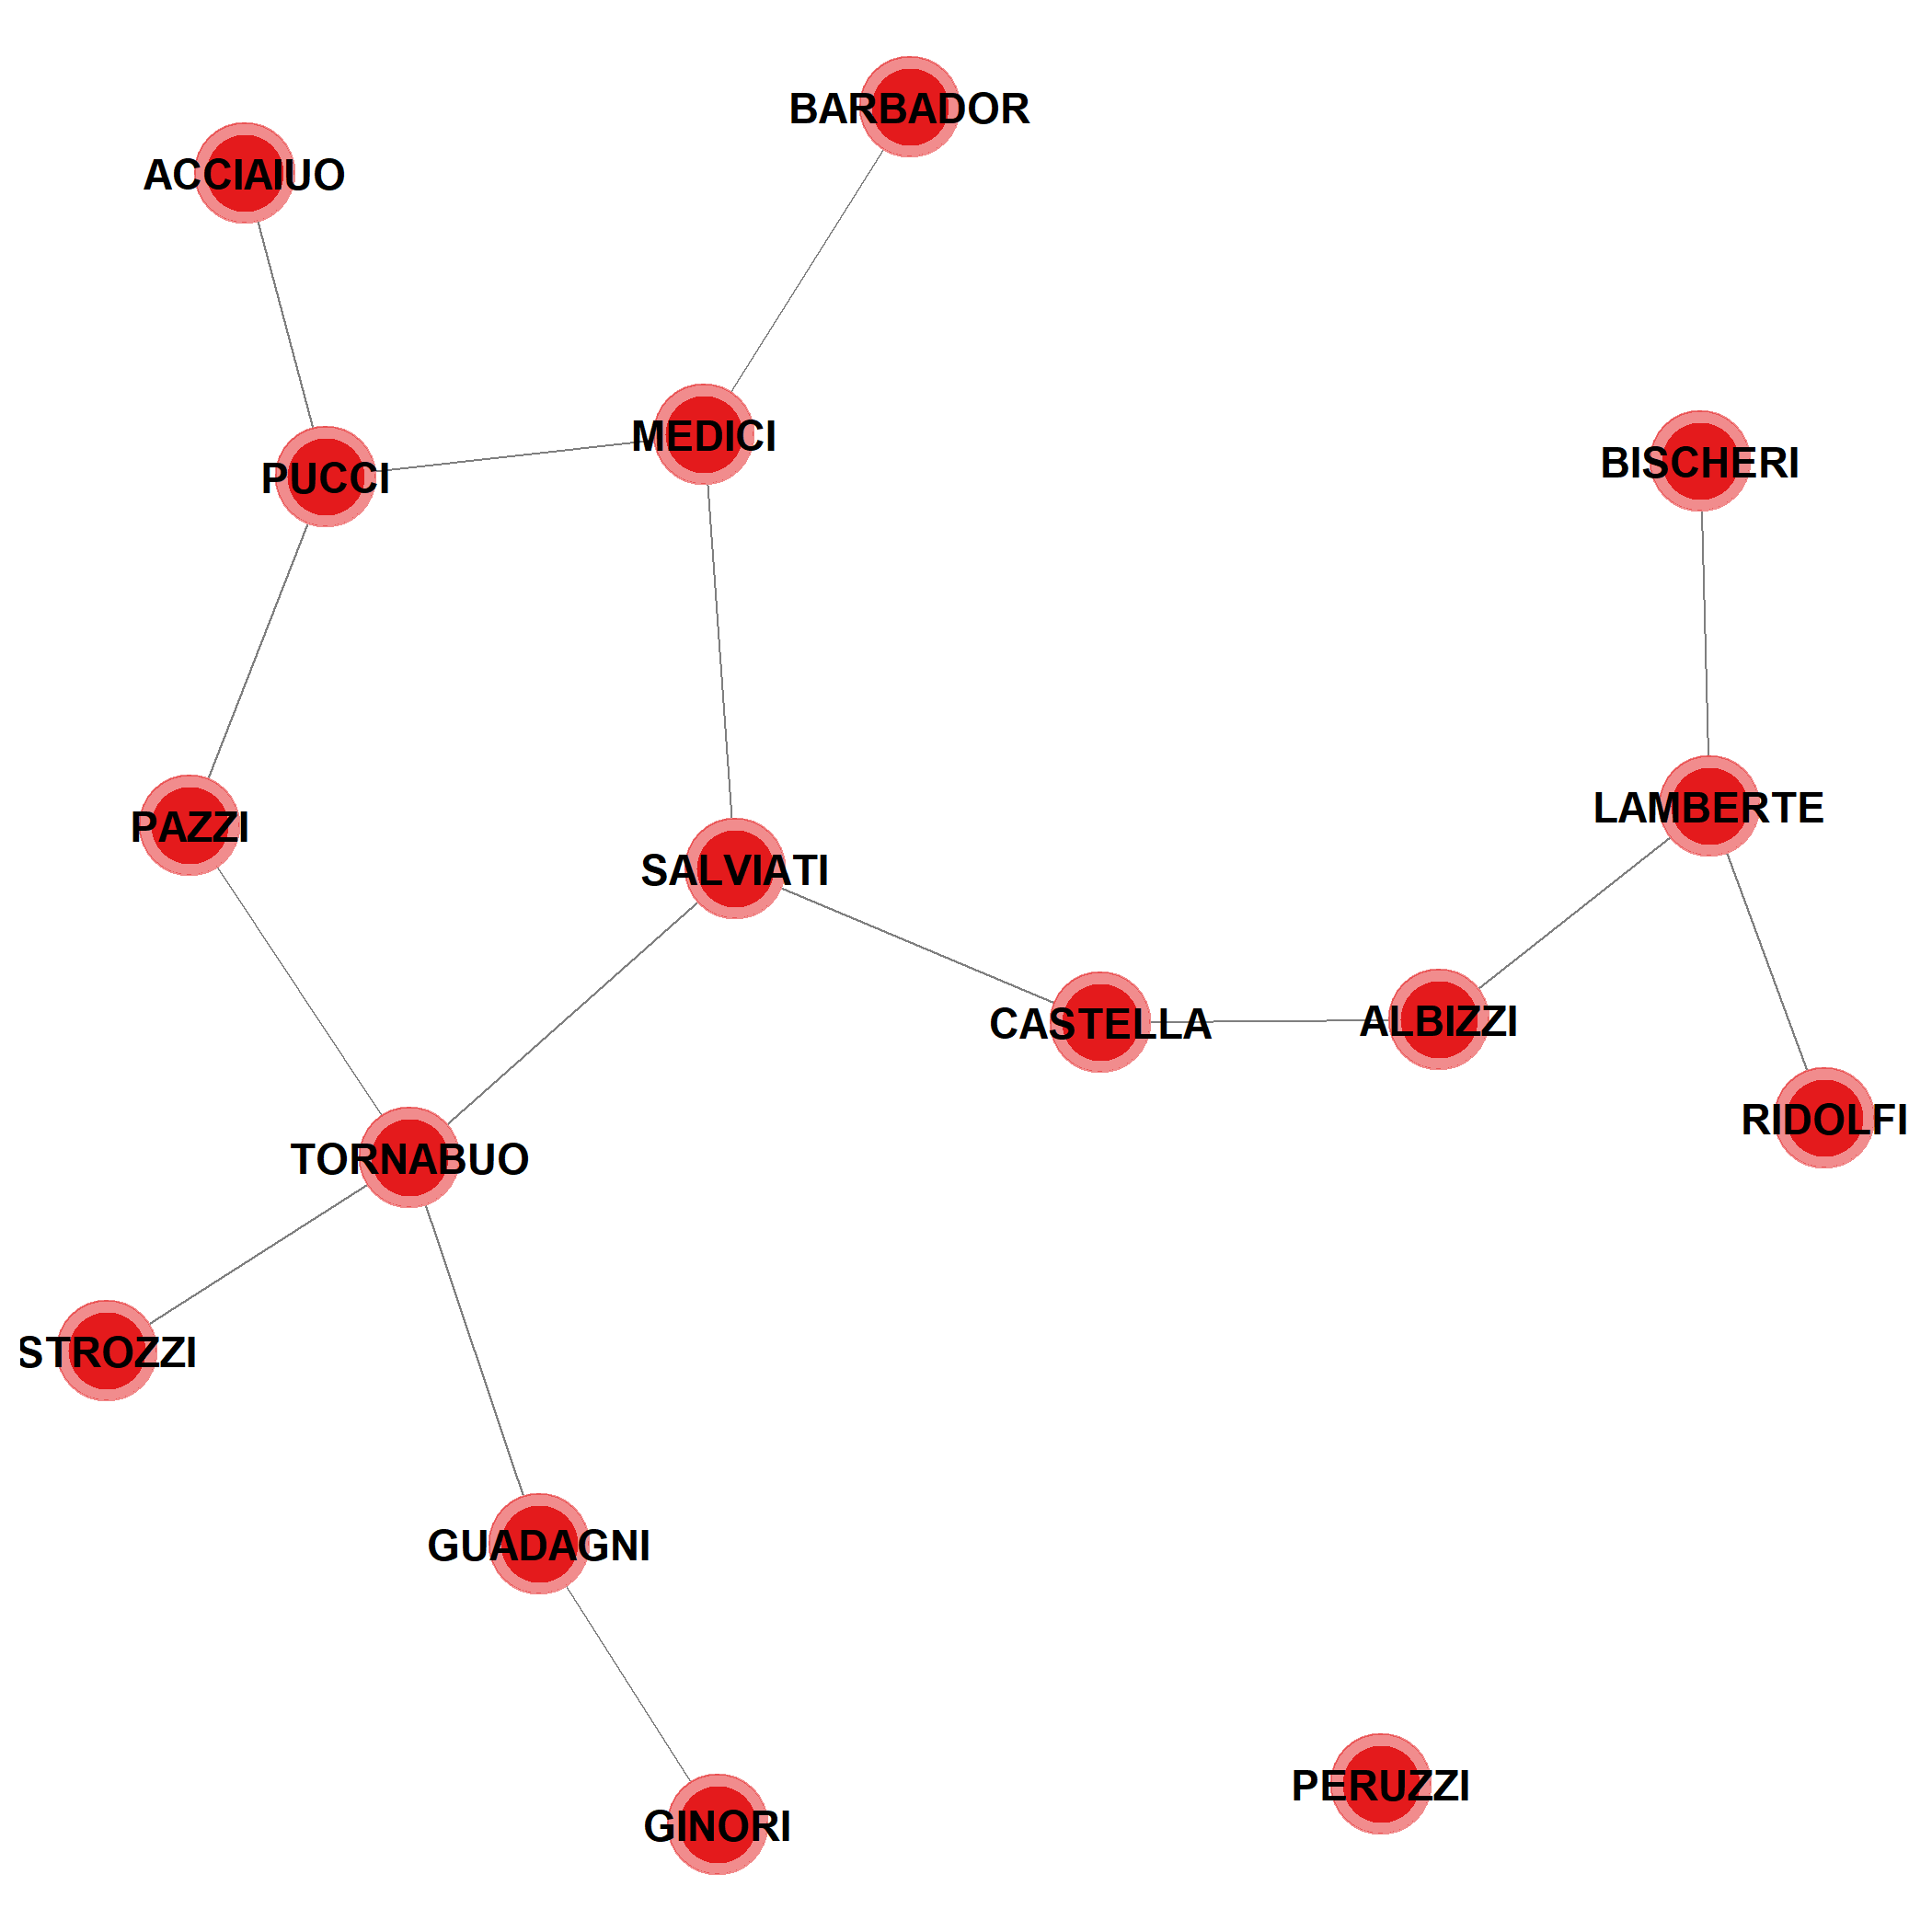
\includegraphics[width=.75\textwidth]{Tesis/Figures/FlorentineSIM.png}
\caption{Simulación de Matrimonio Florentino}
\centering
\end{figure}

También utilizamos las medidas de bondad de ajuste para ver qué tan buena es nuestra estimación. Con esto obtenemos la siguiente tabla de las medidas de bondad de ajuste y las correspondientes gráficas.

\begin{center}
 \begin{tabular}{||c c c c c c||} 
 \hline
 Estadística & obs & min & media & max & Valor p MC \\ [.5ex]
 \hline\hline
 Aristas & 20.00 & 9 & 19.30 & 29 & 1 \\ 
 \hline
 Triángulo & 3 & 0 & 2.67 & 10 & 1 \\
 \hline
\end{tabular}
\end{center}

\begin{figure}[h]
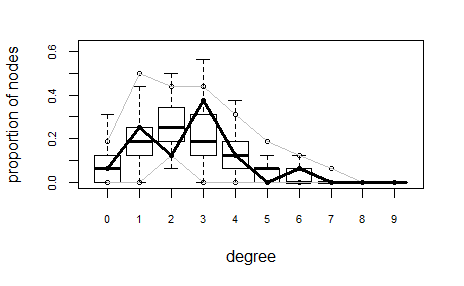
\includegraphics[width=.5\textwidth]{Tesis/Figures/Flo1mc.jpg}
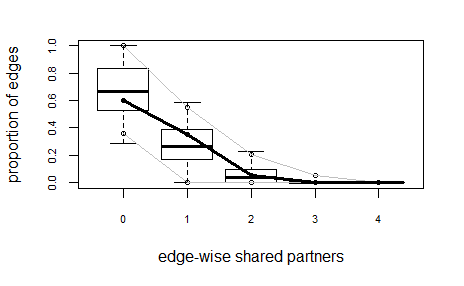
\includegraphics[width=.5\textwidth]{Tesis/Figures/flo2mc.jpg}
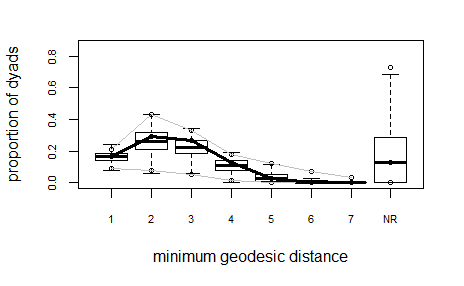
\includegraphics[width=.5\textwidth]{Tesis/Figures/flo3mc.jpg}
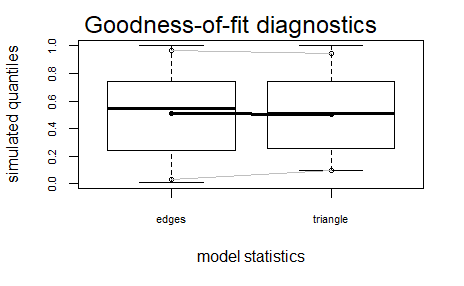
\includegraphics[width=.5\textwidth]{Tesis/Figures/flo4mc.jpg}
\caption{Medidas de Bondad con triángulo}
\centering
\end{figure}

Así que seguimos iterando e implementamos un modelo con otra útil medida de Asociaciones compartidas perimetrales ponderadas geométricamente cuyas estadísticas de descritas por \cite{hunter2007curved} son


\begin{*equation}

\delta w = e^{\alpha}\{1-(1-e^{-\alpha})^1\} \times 3 - e^\alpha{\{1-(1-e^{-\alpha})^0\}} \times 2

\end{*equation}

donde $\alpha$ es el parámetro de la medida de asociaciones compartidas perimetrales ponderadas geométricamente.

Remplazamos la estadística de triángulos por ésta y generamos nuestro modelo. Obtenemos que $\theta_1 = -1.709$ y que $\theta_2 = .1047$ con los siguientes diagnósticos. 

\begin{figure}[h]
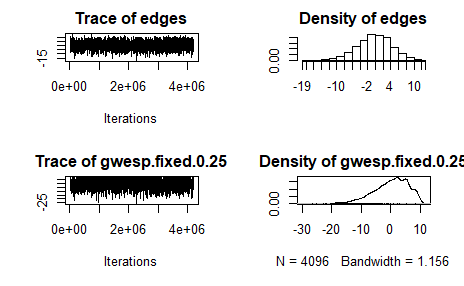
\includegraphics[width=1\textwidth]{Tesis/Figures/mcmcgwesp.jpg}
\caption{Diagnostico MCMC con medida geométrica.}
\centering
\end{figure}

Vemos que éste se ajusta mejor que con los triángulos pero es muy parecido. Con la comparación de las medidas de ajuste y sus correspondientes gráficas de bondad de ajuste en la Figura 5.6 entonces vemos que se ajustan de forma parecida y comparable.

\begin{center}
 \begin{tabular}{||c c c c c c||} 
 \hline
 Estadística & obs & min & media & max & Valor p MC \\ [.5ex]
 \hline\hline
 Aristas & 20.00 & 10 & 19.85 & 34 & 1 \\ 
 \hline
 Gwesp(.25) & 8.221 & 0 & 8.27 & 27.541 & .86 \\
 \hline
\end{tabular}
\end{center}



\begin{figure}[h]
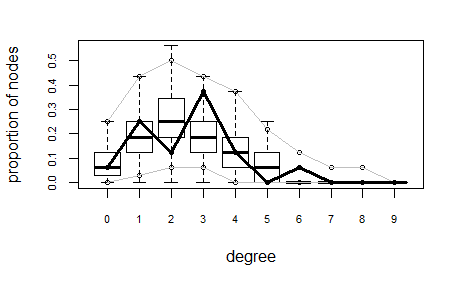
\includegraphics[width=.5\textwidth]{Tesis/Figures/gwespgof1.jpg}
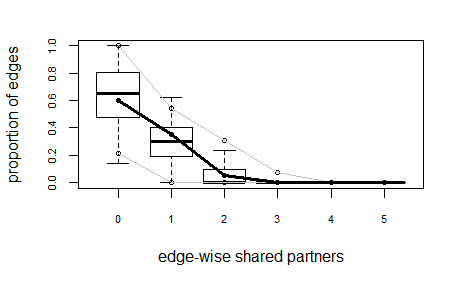
\includegraphics[width=.5\textwidth]{Tesis/Figures/gwespgof2.jpg}
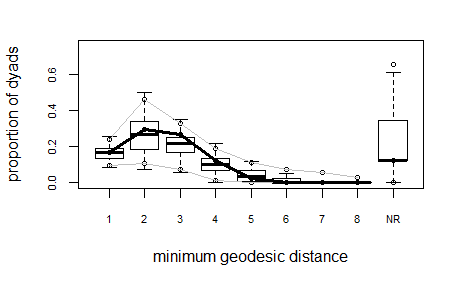
\includegraphics[width=.5\textwidth]{Tesis/Figures/gwespgof3.jpg}
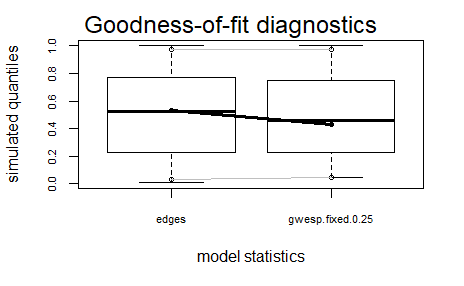
\includegraphics[width=.5\textwidth]{Tesis/Figures/gwespgof4.jpg}
\caption{Medidas de Bondad con GWESP(.25)}
\centering
\end{figure}



\section{Caso de navegación en internet}

Gracias a la generosa ayuda de la empresa Hexagon Data es que tenemos acceso a \textit{Lotame Data Stream} que es un servicio que proporciona acceso en tiempo real a datos de comportamiento sin procesar de cientos de millones de perfiles de navegadores de internet en millones de sitios web. Cada uno de estos registros de millones de \textit{cookies} vienen con información sobre cuándo es que se hicieron una serie de acciones en internet, el país en donde se hicieron, y el sitio web en donde se hicieron. Estos comportamientos entonces están catalogados por Lotame y sus clientes en una taxonomía maestra (ver anexo). Los datos representan el 1\% de todo el tráfico de usuarios de internet en Estados Unidos a través de varias semanas y suman alrededor de 9 millones de usuarios y 1,000 millones de comportamientos registrados. Sin embargo, no todos los comportamientos están catalogados, ya que sólo alrededor del 30$\%$ de la muestra está catalogada dentro de la taxonomía maestra. 

Un registro de una \textit{cookie} cualquiera se ve de la siguiente forma:
\begin{verbatim}
    {"id":{"val":"3c020b70ddec74ed22f6e6e676d2a952",
    "type":"cookie"},
    "country":"US","region":"na",
    "events":[{"tap":"DEVICE","src":"ldxsample1",
    "subSrc":"b590776e","ts":1537056014,
    "add":[8852078,34922299,2296544,41536150,52229337,
           648377,24729307],
    "remove":[33064974,41668881,41668880]}]}
\end{verbatim}

Es decir que este registro viene atado a una \textit{cookie} con id 3c020b70ddec74ed22f6e6e676d2a952 de Estados Unidos con región desconocida. Llevo a cabo su comportamiento en el momento 1537056014 en el sitio web b590776e y fueron 7 interacciones con el sitio web en ese momento. Adicionalmente también se le quitaron 3 comportamientos de forma programada pues no ha repetido esos comportamientos en los últimos 90 días. Sabemos entonces que esta lista de comportamientos están relacionadas a través del usuario. Sin embargo, no queremos relacionar estos identificadores de comportamiento unos con los otros pues son demasiado granulares y son únicos a los sitios web en donde viven. Entonces es que antes de generar una relación entre estos comportamientos es de conveniencia abstraer su significado a los elementos de la taxonomía del mercado de terceros en donde se compra y vende la información de estos usuarios.

Dos registros de la taxonomía del mercado de terceros se ven de la siguiente forma:

\begin{verbatim}
    {"behavior_id":41536150,"hierarchy_nodes
    ":[{"id":52650,
    "path":"Lotame Category Hierarchy^
    Sports & Recreation^Motorsports"}]}
    {"behavior_id":24729307,"hierarchy_nodes"
    :[{"id":525099,
    "path":"Lotame Data Selling Network - Location Hierarchy^
    Countries^North America^United States^Kansas"}]}
\end{verbatim}

Es decir que para el primer registro del \textit{behavior} está asignado al nodo de la taxonomía del mercado de terceros con id 52650  que corresponde al nodo \textit{Lotame Category Hierarchy\textasciicircum Sports & Recreation\textasciicircum Motorsports}. Haciendo este mismo análisis para el segundo registro y comparando con nuestro usuario vemos que nuestro usuario cualquiera está interesado en estos dos comportamientos a la vez. Entonces para la creación de nuestro grafo podemos garantizar que hay al menos una arista entre los nodos de Kansas y de \textit{Motorsports}. 

Así pues en términos matemáticos podemos representar esta relación como  un grafo bipartito en donde se tiene a los nodos de los usuarios de un lado conectados a los distintos nodos categoría de la taxonomía del otro lado. A través de esta representación es que podemos generar un grafo no dirigido en donde las categorías están conectadas entre sí a través del número de usuarios que tienen ambas categorías en su lista de comportamientos clasificados.

\begin{minipage}{1\linewidth}
\begin{figure}[H]\centering

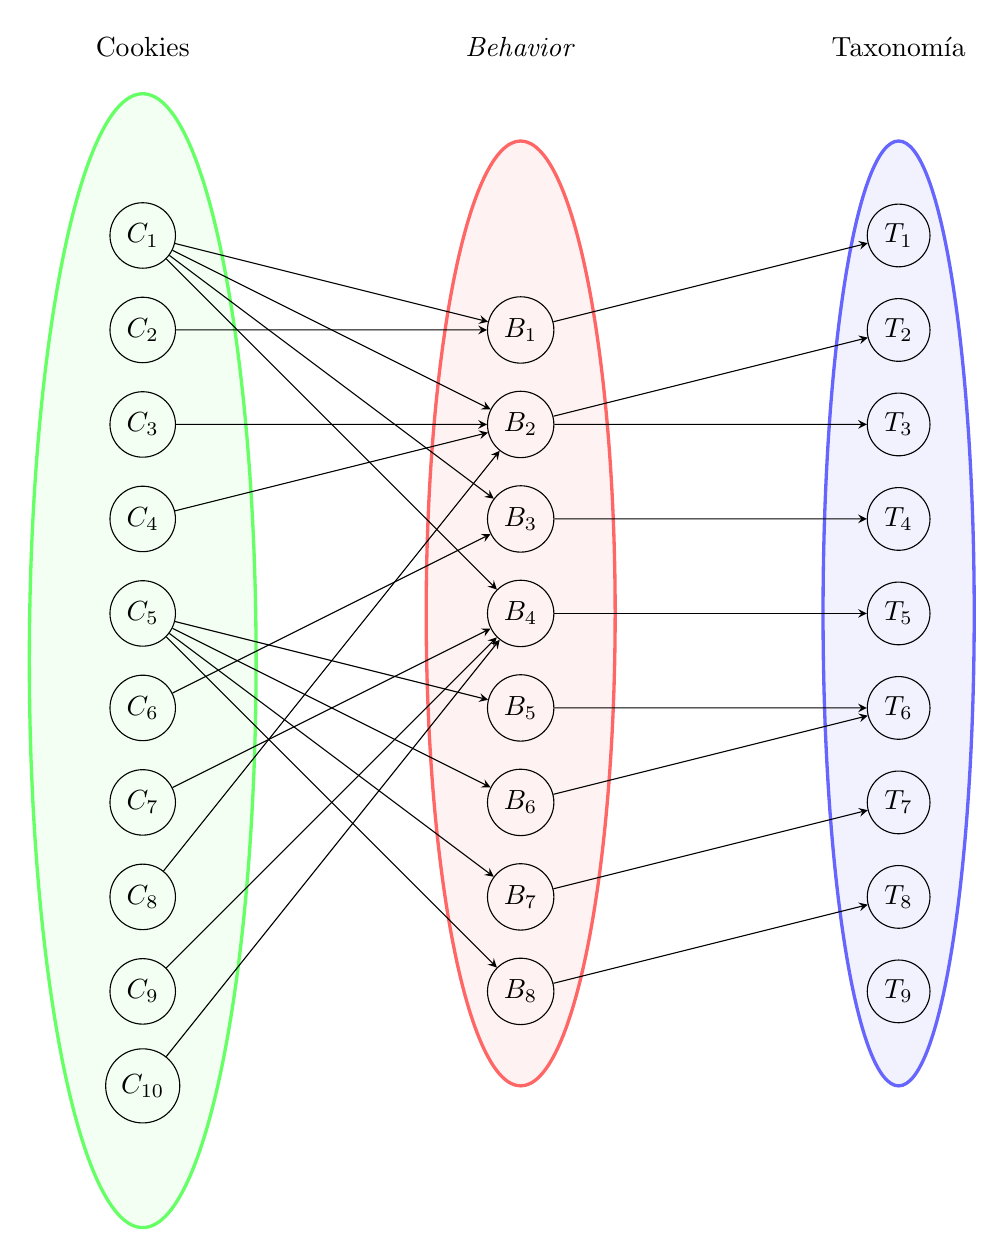
\begin{tikzpicture}[ scale=1.2]
\tikzset{vertex/.style = {shape=circle,draw,minimum size=2.2em}}
\tikzset{edge/.style = {->,> = latex}}


\filldraw[color=green!60, fill=green!5, very thick](0,-.5) ellipse (1.2 and 6);
\filldraw[color=red!60, fill=red!5, very thick](4,0) ellipse (1 and 5);
\filldraw[color=blue!60, fill=blue!5, very thick](8,0) ellipse (.8 and 5);


% vertices
% 
\node[vertex] (a) at (4,3) {$B_1$};
\node[vertex] (b) at (4,2) {$B_2$};
\node[vertex] (c) at (4,1) {$B_3$};
\node[vertex] (d) at (4,0) {$B_4$};
\node[vertex] (e) at (4,-1) {$B_5$};
\node[vertex] (e1) at (4,-2) {$B_6$};
\node[vertex] (e2) at (4,-3) {$B_7$};
\node[vertex] (e3) at (4,-4) {$B_8$};


\node[vertex] (g) at (0,4) {$C_1$};
\node[vertex] (h) at (0,3) {$C_2$};
\node[vertex] (i) at (0,2) {$C_3$};
\node[vertex] (j) at (0,1) {$C_4$};
\node[vertex] (k) at (0,0) {$C_5$};
\node[vertex] (l) at (0,-1) {$C_6$};
\node[vertex] (m) at (0,-2) {$C_7$};
\node[vertex] (n) at (0,-3) {$C_8$};
\node[vertex] (o) at (0,-4) {$C_9$};
\node[vertex] (p) at (0,-5) {$C_{10}$};


\node[vertex] (g1) at (8,4) {$T_1$};
\node[vertex] (h1) at (8,3) {$T_2$};
\node[vertex] (i1) at (8,2) {$T_3$};
\node[vertex] (j1) at (8,1) {$T_4$};
\node[vertex] (k1) at (8,0) {$T_5$};
\node[vertex] (l1) at (8,-1) {$T_6$};
\node[vertex] (m1) at (8,-2) {$T_7$};
\node[vertex] (n1) at (8,-3) {$T_8$};
\node[vertex] (o1) at (8,-4) {$T_9$};


\node (w) at (0,6) {Cookies};
\node (x) at (4,6) {\textit{Behavior}};
\node (x) at (8,6) {Taxonomía};


\path[-stealth] (g) edge (a);
\path[-stealth] (g) edge (b);
\path[-stealth] (g) edge (c);
\path[-stealth] (g) edge (d);
\path[-stealth] (h) edge (a);
\path[-stealth] (i) edge (b);
\path[-stealth] (j) edge (b);
\path[-stealth] (k) edge (e);
\path[-stealth] (k) edge (e1);
\path[-stealth] (k) edge (e2);
\path[-stealth] (k) edge (e3);
\path[-stealth] (l) edge (c);
\path[-stealth] (m) edge (d);
\path[-stealth] (n) edge (b);
\path[-stealth] (o) edge (d);
\path[-stealth] (p) edge (d);
%\path[-stealth] (b) edge (g);


\path[-stealth] (a) edge (g1);
\path[-stealth] (b) edge (h1);
\path[-stealth] (b) edge (i1);
\path[-stealth] (c) edge (j1);
\path[-stealth] (d) edge (k1);
\path[-stealth] (e) edge (l1);
\path[-stealth] (e1) edge (l1);
\path[-stealth] (e2) edge (m1);
\path[-stealth] (e3) edge (n1);

%\draw (4,4) node[cross=8pt,red] {};


%\draw (0.2,8)--(3.8,8);



\end{tikzpicture}
\caption{ Representación de las relaciones }
\end{figure}
\end{minipage}


Vale la pena notar la relación entre \textit{behavior} y los nodos de la taxonomía puede ser de uno a muchos. Darle clic a un artículo cuyo título es \textbf{presidente propone la cancelación de los puentes} puede tener asociado los temas de Política, Turismo y México. En la Figura 5.1 podemos observar que $T_6$ y $T_7$ y $T_{8}$  están relacionados a través de $C_5$. Al igual que $T_1, T_2, T_3,T_4$ y $T_5$ están relacionados a través de $C_1$


Sin embargo, la taxonomía tiene más de 5000 nodos categoría cuando la tomamos en su forma original. Sin embargo dada la estructura jerárquica de la taxonomía es que podemos ""subirla de nivel"" para reducir el número de nodos. Por ejemplo, podríamos en vez de tomar el nodo en la taxonomía de \textit{Lotame - Media & Entertainment - Sports - Team Sports - Football Soccer - International Competiton} podemos decidir catalogarlo simplemente como \textit{Lotame - Media & Entertainment - Sports - Team Sports - Football Soccer}. Sin embargo, perdemos cierto nivel de granularidad. Para esta tesis se hizo un desglose artesanal de cada tipo de comportamiento de acuerdo a su naturaleza para reducir el número de nodos categoría pero aún manteniendo una estructura general fiel al contenido de la taxonomía original.

Los modelos de grafos exponenciales tienen muchas formas y la cantidad de teoría detrás de cada tipo de modelaje como el ajuste del modelo a través del tiempo con grafos temporales o en este caso utilizando el grafo que es generado con los usuarios como nodos conectados por sus comportamientos durante un periodo en el tiempo. También sería posible crear un grafo en donde se usen los sitios web en donde sucedieron los comportamientos catalogados conectados con aristas basadas en el contenido, y así medir y predecir la cercanía en el contenido de distintos sitios web. 

\subsubsection{Nuestros Nodos Construidos}

Para simplificar nuestro caso restringimos el número de nodos de nuestro grafo para que estén limitados a intereses, \textit{hobbies} y medios. Es decir que los nodos que se refieren a información tecnográfica (con excepción del sistema operativo) y geográfica han sido eliminados para reducir de forma drástica la complejidad del problema y de esta forma de más de cinco mil nodos de la taxonomía es que tenemos un caso donde tenemos alrededor de 729 nodos de donde viene información más general. Sin embargo, el grafo generado con las categorías de estas taxonomías consiste de al menos dos subgrafos inducidos que no comparten ninguna arista entre ellos; en realidad hay muchos nodos totalmente desconectados. Por lo tanto el modelo de ERGMs solamente se corrió sobre el subgrafo máximo inducido de los presentes.


\subsection{Explorando las propiedades de nuestro grafo}


Nuestra muestra proviene del muestreo de la unidad de tiempo UNIX 1536267600 equivalente a 06/09/2018 a las 9:00 a.m. hasta tiempo UNIX 1537286399 equivalente a  18/09/2018 a las 3:59 p.m. de donde la matriz de adyacencia que fue obtenida del muestreo de combinaciones en dos. Se procesaron alrededor de 38.4762 GB de datos comprimidos de \textit{streaming} en el periodo mencionado o alrededor de 25,435,675 registros individuales con los cuales se hicieron las combinaciones. Los \textit{scripts} de Python utilizados para la extracción de la información de los  del \textit{stream} y el algoritmo para la creación de las aristas entre los nodos de contenido viene anexado de igual forma y entrega listas de aristas. El código de R para la manipulación de las tablas para convertir 
los datos a objetos de \textit{network} en R y para el modelaje de \textit{ERGMs} en \textit{statnet} también viene anexado. 

Desafortunadamente, el grafo generado de 729 nodos que está aquí ilustrado con colores del nodo que indican sus categorías en general se encuentra desconectado como ya fue mencionado. El grafo original contiene 111,131 aristas es decir que tiene una densidad de 0.209. 

\begin{figure}[!ht]
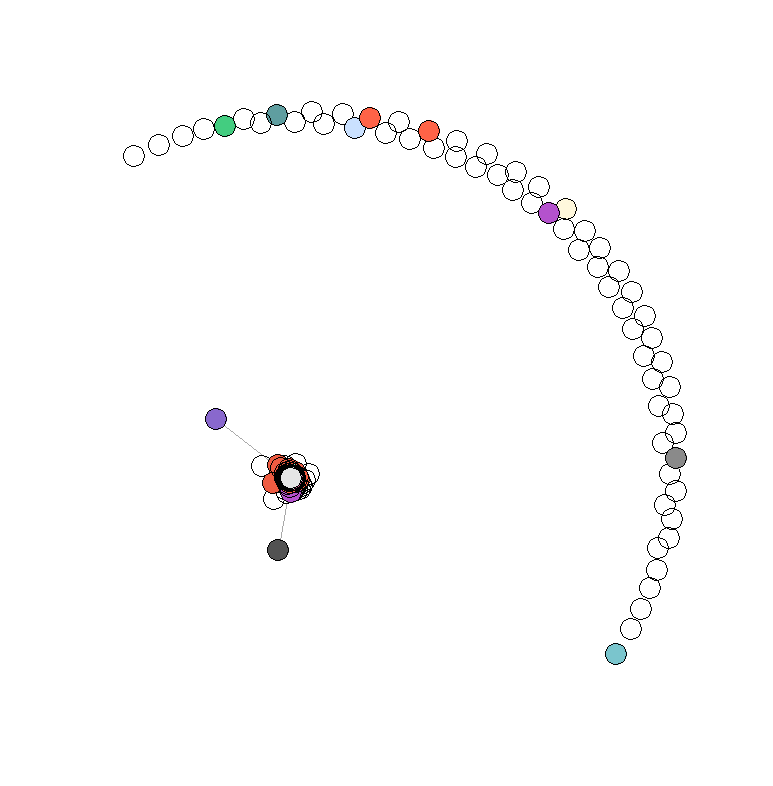
\includegraphics[width=1\textwidth]{Tesis/Figures/LotameFull.png}
\caption{Grafo de las cookies completo de Lotame con colores por tema.}
\centering
\end{figure}

Para el modelo en realidad vamos a elegir el subgrafo inducido y vamos a eliminar las aristas de peso del cuartil más chico para sólo quedarnos con las aristas que tienen mayor interacción, entonces eliminamos todas las aristas de peso menor a 46. El peso de cada arista se determinó a partir del número total de \textit{cookies} que tenían ambos comportamientos en sus eventos. La mediana del peso de las aristas entonces fue de 145 y el mayor peso reportado de 2,068,796 entre los nodos 52200 y 52413, que son el \textit{Lotame Category Hierarchy - Fashion & Beauty-Clothing} y \textit{Lotame Category Hierarchy - Health & Medicine - Physical Fitness} respectivamente. Una mejora posible en el muestreo sería diagnosticar cuáles usuarios en realidad son \textit{bots} que recorren una gran parte del contenido del grafo completo y eliminarlos del muestreo pero esto está fuera del alcance de esta tesis. A continuación se encuentra el histograma del log peso de las aristas en el grafo antes de hacer el filtro del cuartil más bajo y elegir el subgrafo inducido mas grande.

\begin{figure}[!ht]
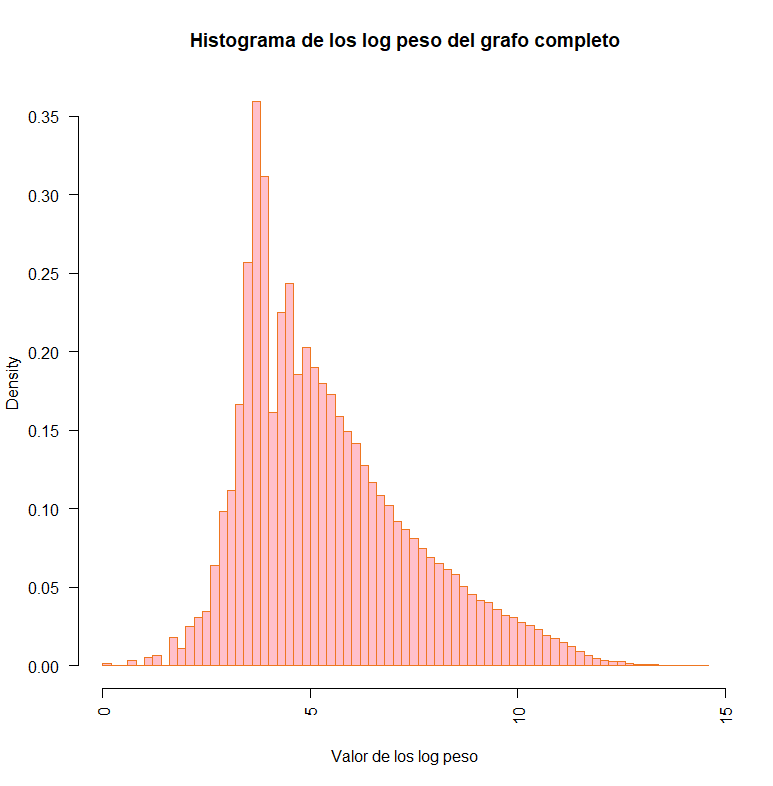
\includegraphics[width=1\textwidth]{Tesis/Figures/HistGrafoCompleto.png}
\caption{Histograma de $\log$ peso del grafo completo de las \textit{cookies} de Lotame.}
\centering
\end{figure}

Entonces nuestro grafo final cuenta con 662 nodos, cuyos elementos se encuentran anexados al final de esta tesis. Cuenta con 84580 aristas es decir que tiene una densidad de 0.193 y podemos dormir tranquilos que al menos esa estadística global es comparable a la de nuestro grafo original. Sin embargo el comportamiento de decadencia exponencial en los pesos de las aristas se ve mucho mejor con la muestra reducida.

\begin{figure}[!ht]
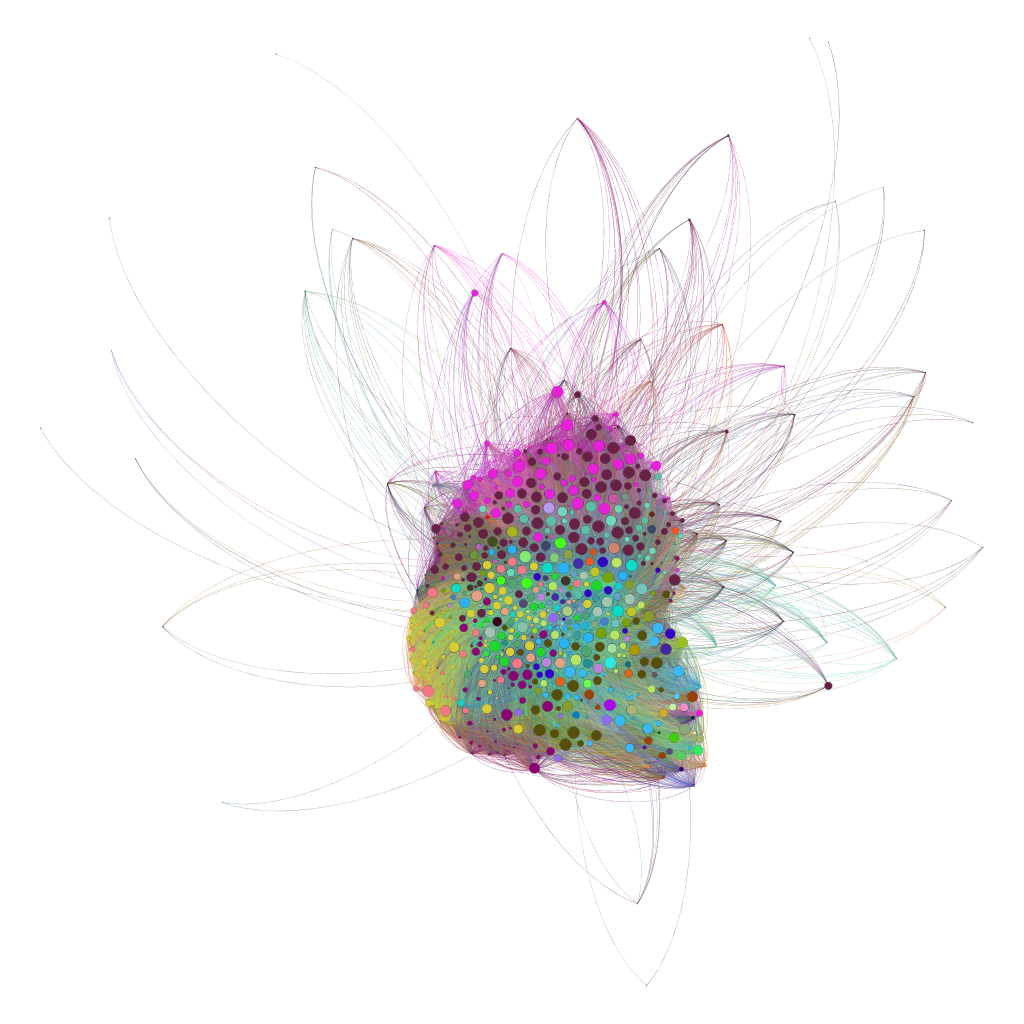
\includegraphics[width=1\textwidth]{Tesis/Figures/LotameFullgraphAmazing.png}
\caption{Subgrafo inducido de la muestra filtrada ordenado por categorías por color y ordenados principalmente con \textit{Force Atlas}.}
\centering
\end{figure}

\begin{figure}[!ht]
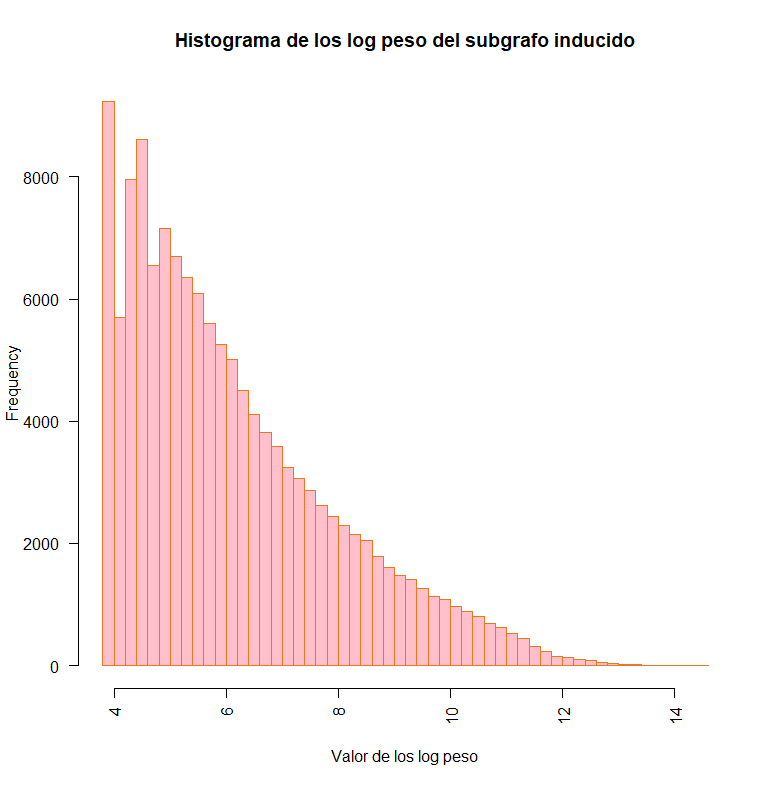
\includegraphics[width=1\textwidth]{Tesis/Figures/HistSubgrafoInducido.png}
\caption{Histograma de $\log$ peso del subgrafo inducido de las cookies de Lotame.}
\centering
\end{figure}
\clearpage

\begin{figure}
 \begin{adjustwidth}{-3.6cm}{}
 \begin{tabular}{||C{2em} C{1em}||}
 \hline
 Nodo & Nodo \\ 
 \hline\hline
Computers and Technology-Operating \\
systems	&	Mobile  Wireless Devices-
Mobile Phones	\\
 \hline
 Fashion and \\
Beauty-Clothing	&	Health and Medicine-Physical Fitness	\\
 \hline
Home and Family-Lawn and \\
Garden	& Home and Family-Home Improvement	\\
\hline
Travel-Business Travel	& Physical Fitness	\\
\hline
Purchase Intent-Food, Beverages and \\
Tobacco-Food Items	&	Health and Medicine	\\
\hline
Purchase Intent-\\
Food, Beverages and Tobacco-\\
Food Items	&	Home and Family-
Lawn and Garden	\\
\hline
Purchase Intent-\\
Food, Beverages and Tobacco-\\
Food Items	&	Food and Beverages-
Recipes and Cooking	\\
\hline
Purchase Intent-\\
Food, Beverages and Tobacco-
Food Items	& Literature-Books	\\
\hline
Lawn and Garden	&	Home Improvement\\ [4ex] 

 \hline
\end{tabular}


 \end{adjustwidth}
 \caption{Los nodos con mayor número de conexiones por usuarios entre ellos.}
\end{figure}











\subsection{Propuesta de distintos modelos}

Aunque empezamos de la misma forma que en el caso florentino en donde tenemos que

\begin{equation*}
    \textit{Lotame} \sim \textit{Numero.de.Aristas}
\end{equation*}

\begin{equation*}
    \log \left( \exp \left( \theta ^ { \prime } g ( y ) \right) \right) = \theta _ { 1 }  \sum _ { i , j > i \in \mathcal{N} } y _ { i j }.    
\end{equation*}

El modelo Bernoulli fracasó y nos indica que esta estadística del grafo se encuentra en el máximo utilizando la estimación de la máxima pseudo verosimilitud.




\begin{equation*}
    \textit{Lotame} \sim  \textit{Numero.de.Triángulos+Numero.de.Aristas}
\end{equation*}

\begin{equation*}
    \log \left( \exp \left( \theta ^ { \prime } g ( y ) \right) \right) =  \theta_1    \times \sum _ { i j k }  y _ { i j } y _ { j k } y _ { k i } 
\end{equation*}



% \begin{equation*}
% \begin{split}
%     &= \exp (0.2325684) /(1+\exp (0.2325684 ))\\
%     &= 0.387
% \end{split}
% \end{equation*}

Después de un poco de exploración de datos y con los diagnósticos de Markov obtenidos para los valores de los parámetros de $\theta_1 = 0.02168062$ y $\theta_2 = -3.26154720$ sospechamos que necesitamos una mejor estadística que éstas para este grafo. Podemos observar los diagnósticos de las cadenas de Markov Monte Carlo en la figura 5.13 y no se ven muy bien. Detenemos el analisis de este modelo y proponemos el modelo con la medida de estrellas alternantes definida en \cite{Snidjers2006}.

\begin{figure}[!ht]
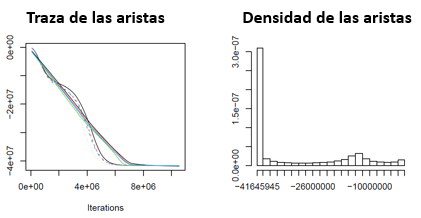
\includegraphics[width=1\textwidth]{Tesis/Figures/mcmc_1.PNG}
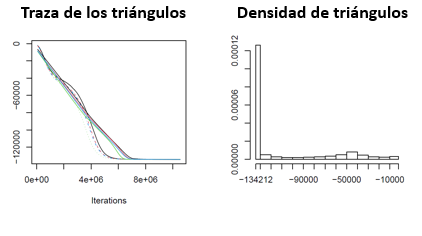
\includegraphics[width=1\textwidth]{Tesis/Figures/mcmc_2.PNG}

\caption{Diagnósticos de Markov del modelo de Triángulos y Aristas.}
\centering
\end{figure}

¡Eureka! Nuestro modelo converge en los valores de $\theta_1 = 16.5167$ y $\theta_2 = -15.2282$ y cuya constante de normalización es $\lambda = 0.5574$. Los diagnósticos de Monte Carlo de la Figura 5.13 se ven bien, pensando que la covariabilidad que se observa entre la traza de aristas y de estrellas alternantes es esperada por \cite{GoodOfFitSocialNetwork}, pues este modelo es equivalente al de los pesos geométricos por razones obvias. Parece que las medidas de bondad de ajuste también parecen ser capaces de ser relativamente buenas para imitar al menos algunos atributos globales de forma parecida a nuestro grafo original. Ver la figura 5.15 para inspeccionar las estadísticas de la bondad de ajuste.

\begin{figure}[!ht]
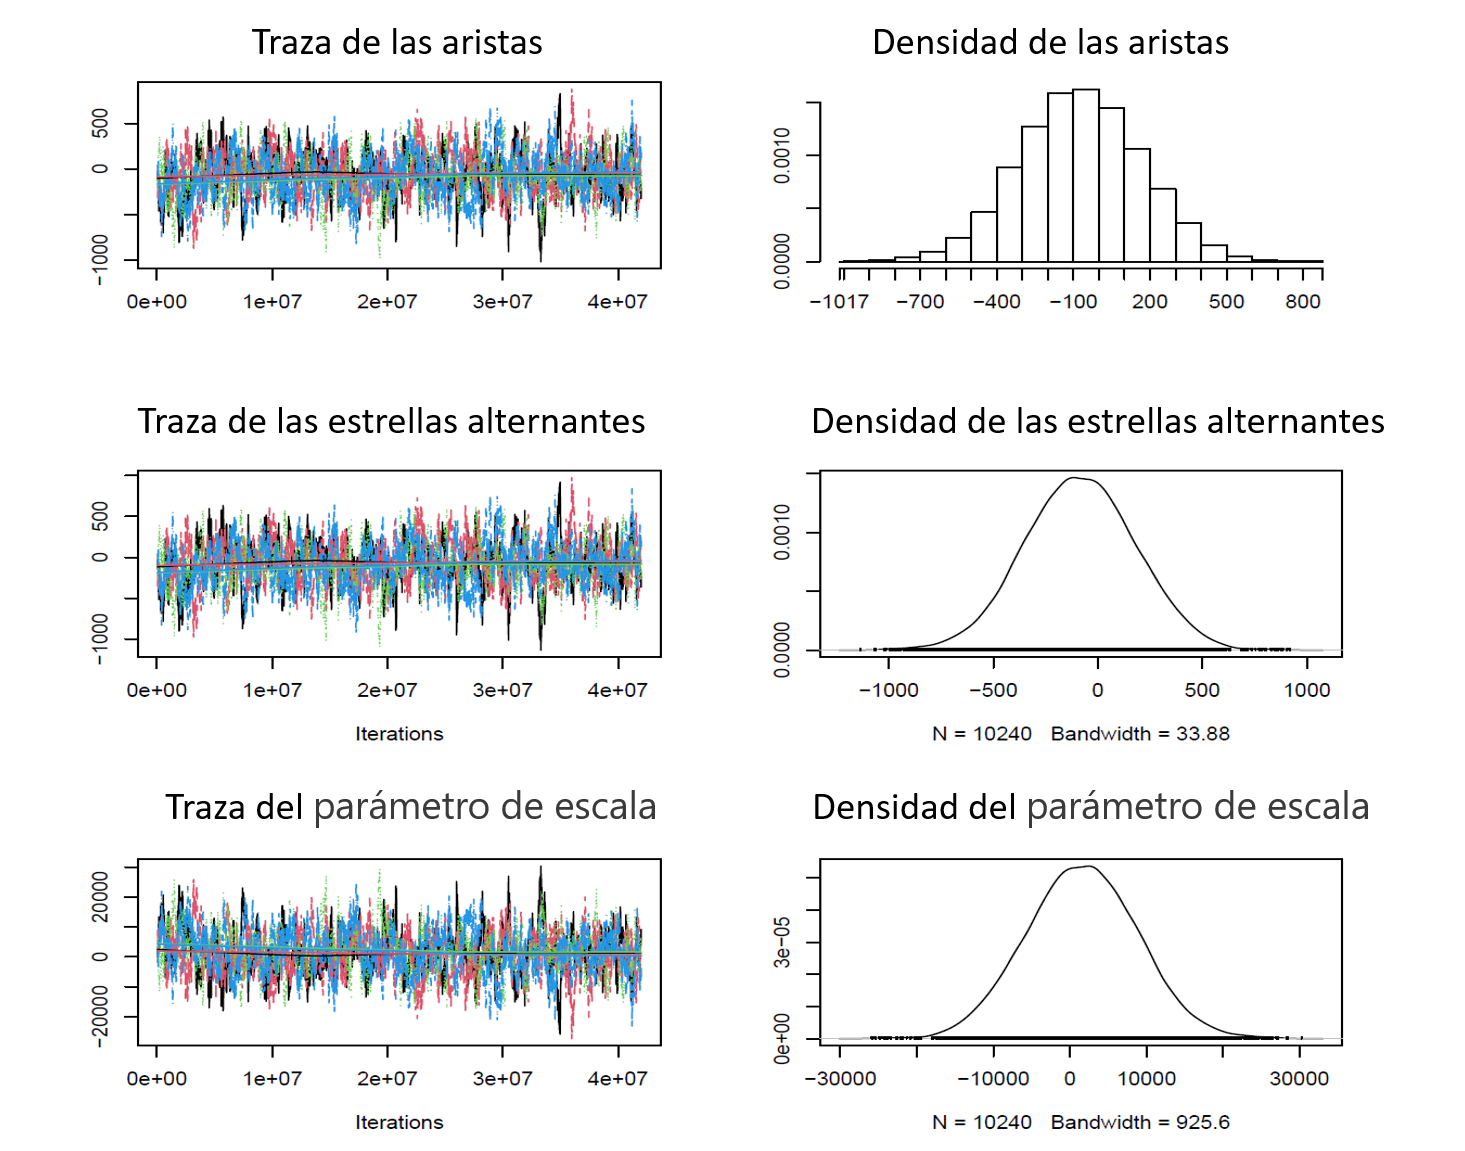
\includegraphics[width=1\textwidth]{Tesis/Figures/mcmc3.PNG}
\caption{Diagnósticos de Markov del modelo de Triángulos y Aristas.}
\end{figure}

\begin{figure}[!ht]
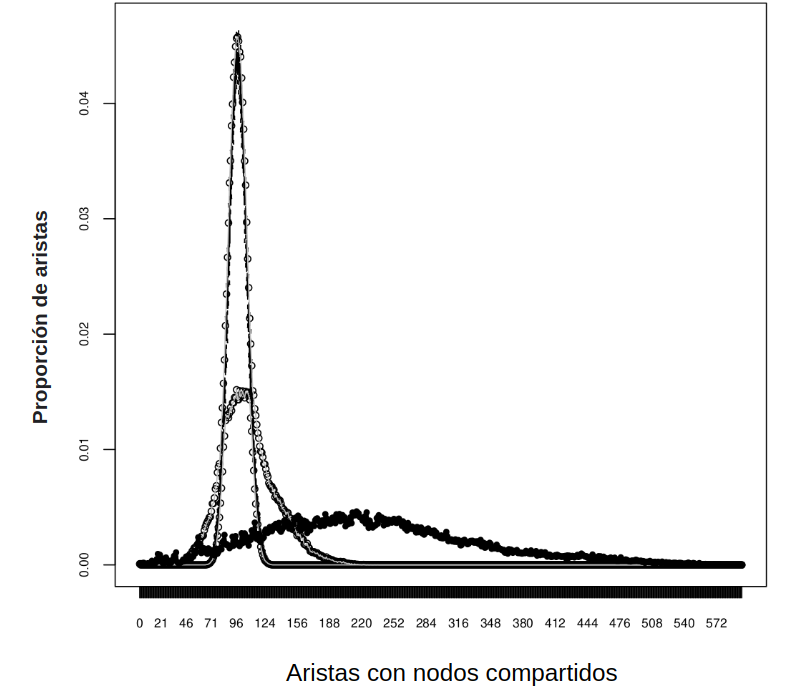
\includegraphics[width=.5\textwidth]{Tesis/Figures/gof_1_aristas_nodos_compartidos.png}
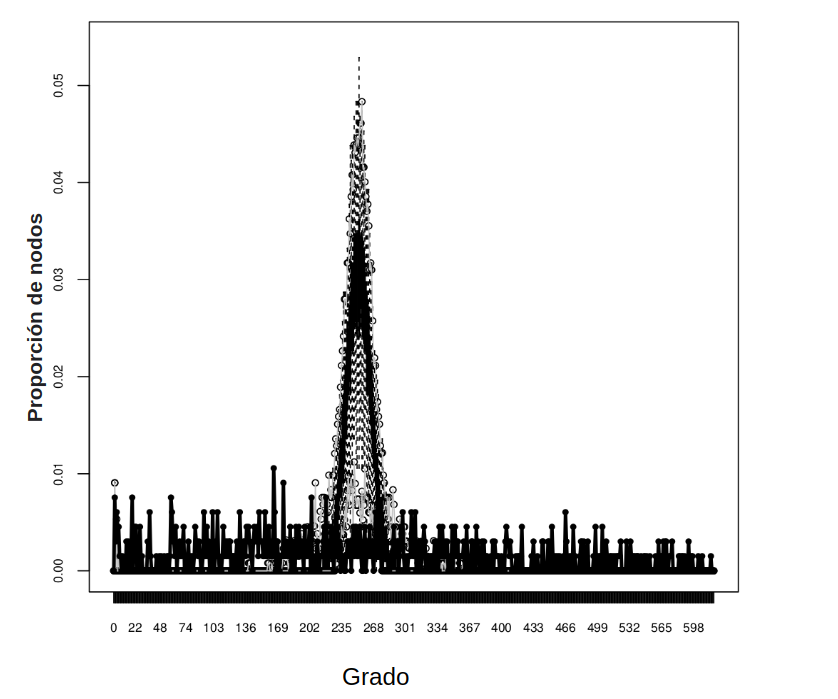
\includegraphics[width=.5\textwidth]{Tesis/Figures/gof_1_degree.png}
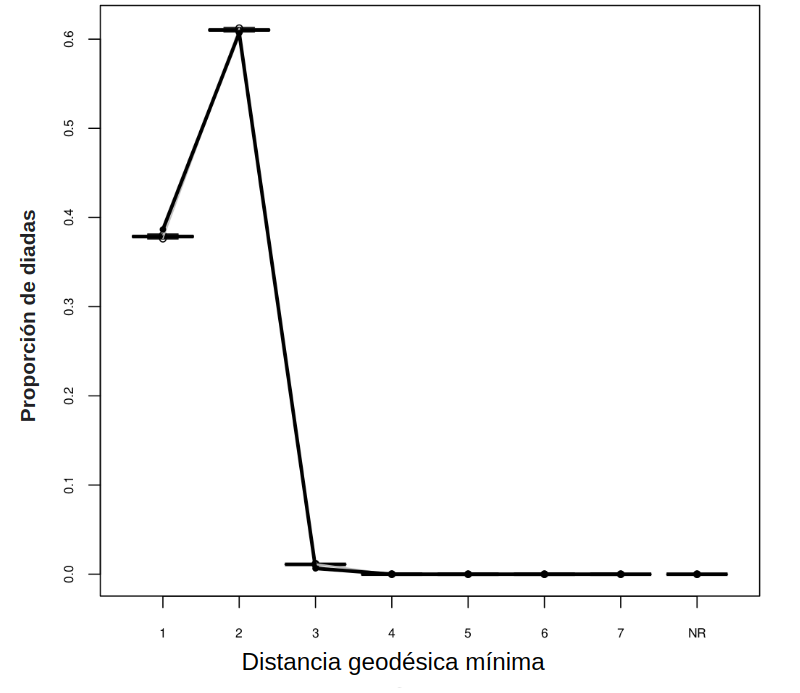
\includegraphics[width=.5\textwidth]{Tesis/Figures/gof_1_distancia.png}
\caption{Medidas de bondad de ajuste del modelo de aristas y Triángulos Estrellas Alternantes}
\end{figure}

De forma adicional también proponemos un modelo en donde podemos incluir información de nuestros nodos con la medida de coincidencia de nodos en temas en general y otro con la especificación de temas en específico cuya clasificación se encuentra en el anexo de esta tesis.

\begin{equation*}
    \textit{Lotame} \sim \textit{Numero.de.Triángulos}+\textit{Estrellas.Alternantes}+
    
    \newline
    \hspace*{2.5cm}\textit{Coincidencia.De.Tema.En.General}
\end{equation*}

y

\begin{equation*}
    \textit{Lotame} \sim \textit{Numero.de.Triángulos}+\textit{Estrellas.Alternantes}+
    
    \newline
    \hspace*{2.5cm} \textit{Coincidencia.De.Tema.En.Específico}
\end{equation*}

cuyos diagnósticos de Markov se encuentran en la Figura 5.16 y 5.17 y cuyos valores de estadísticas son respectivamente $\theta_1 = 125.3$ y $\theta_2 = -124.3$ y $\theta_3 = .5056$ con constante de normalización de $\lambda = .009292$ y $\theta_1 = 16.51799$ y $\theta_2 = -15.22960$ y $\theta_3 = 0.21229$ y cuya constante de normalización es $\lambda = 0.55746$. Vale la pena notar que en el caso de coincidencia de nodos en general las estadísticas de aristas y estrellas alternantes son significativas pero la coincidencia de género en general no lo es. Por el otro lado en el caso de coincidencia de género específico tenemos que las estadísticas de aristas y estrellas alternantes no son significativas pero la de coincidencia de género en específico sí lo es. Además podemos ver que en el caso de la coincidencia de aristas específicas todos los valores de las estadísticas están centradas alrededor de 0. Una interpretación de esto es que utilizando la coincidencia de género especifica nuestro grafo únicamente se conecta utilizando el criterio que sí los nodos comparten el mismo tema en específico o sí es que no. Por el otro lado en el caso en general vemos que parece ser que las estadísticas de aristas y estrellas alternantes determinan la forma en la cual los nodos se conectan mientras que la coincidencia de género únicamente da un poco de forma a la cual nuestro grafo se realiza.

\begin{figure}[!ht]
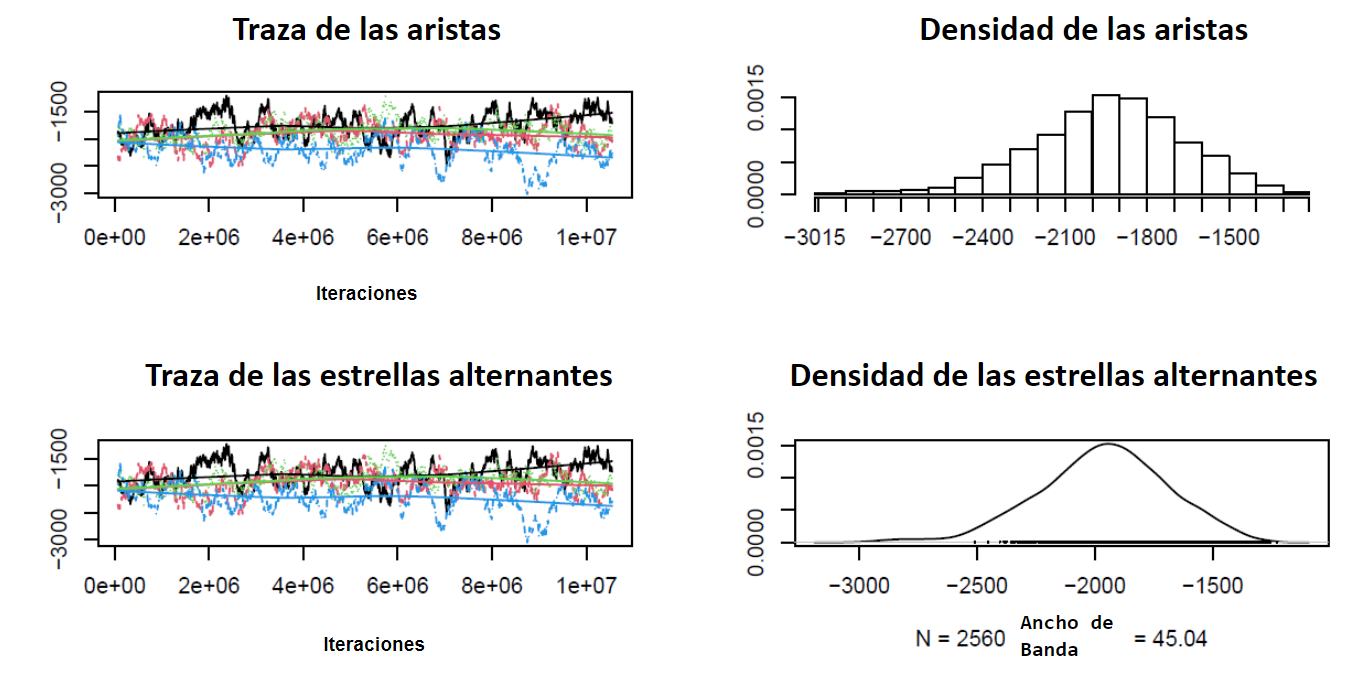
\includegraphics[width=1\textwidth]{Tesis/Figures/mcmc_general1.PNG}
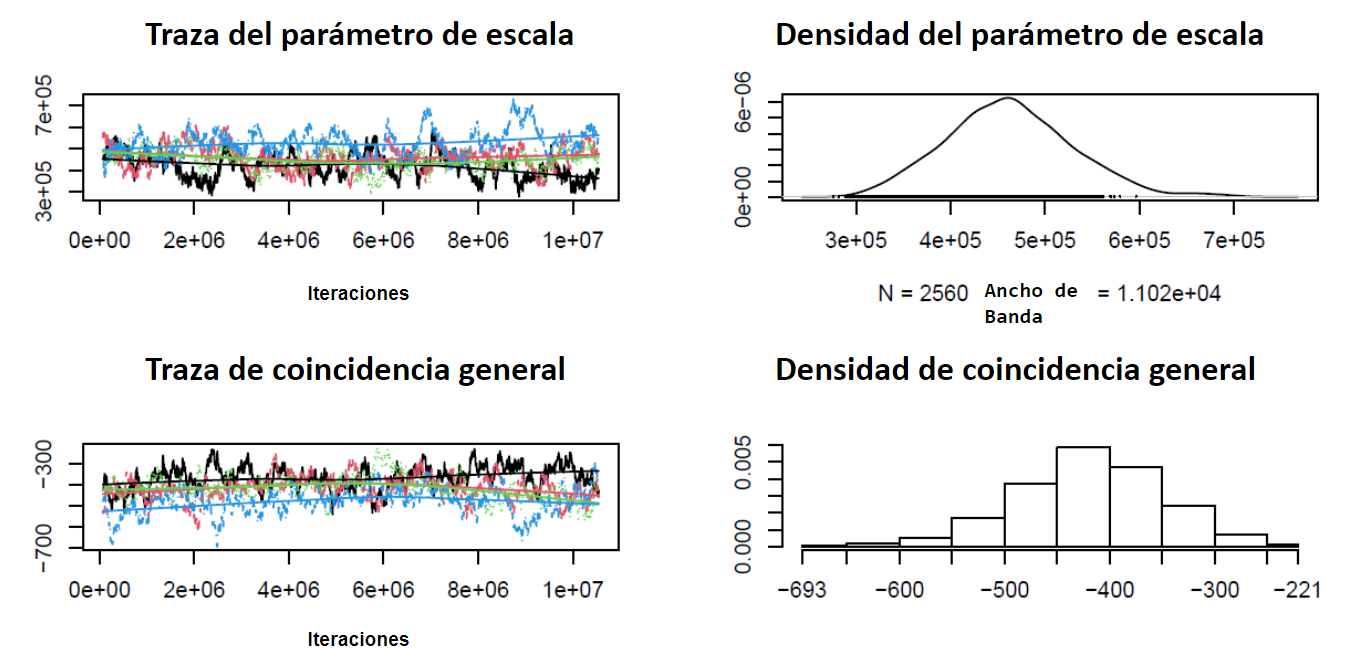
\includegraphics[width=1\textwidth]{Tesis/Figures/mcmc_general2.PNG}
\caption{Diagnósticos de Markov del modelo de Triángulos Estrellas Alternantes y coincidencia de género general}
\end{figure}


\begin{figure}[!ht]
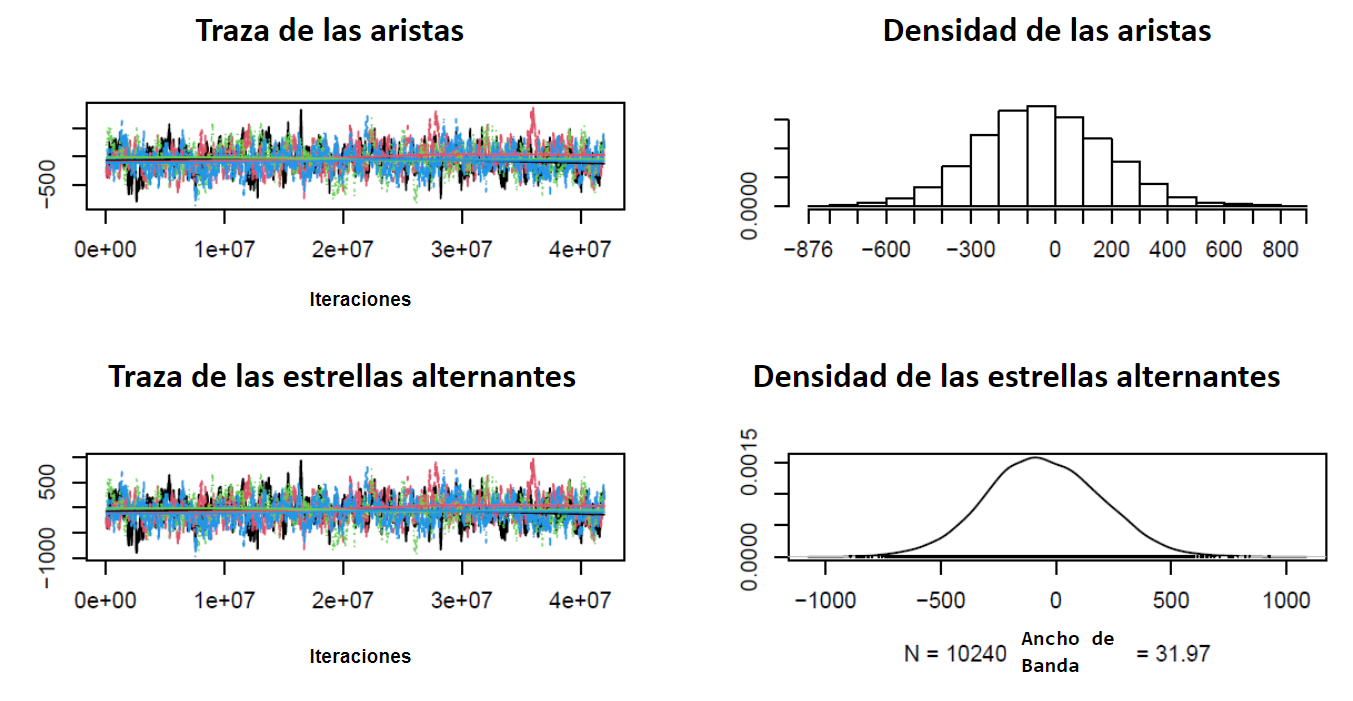
\includegraphics[width=1\textwidth]{Tesis/Figures/mcmc_specific1.PNG}
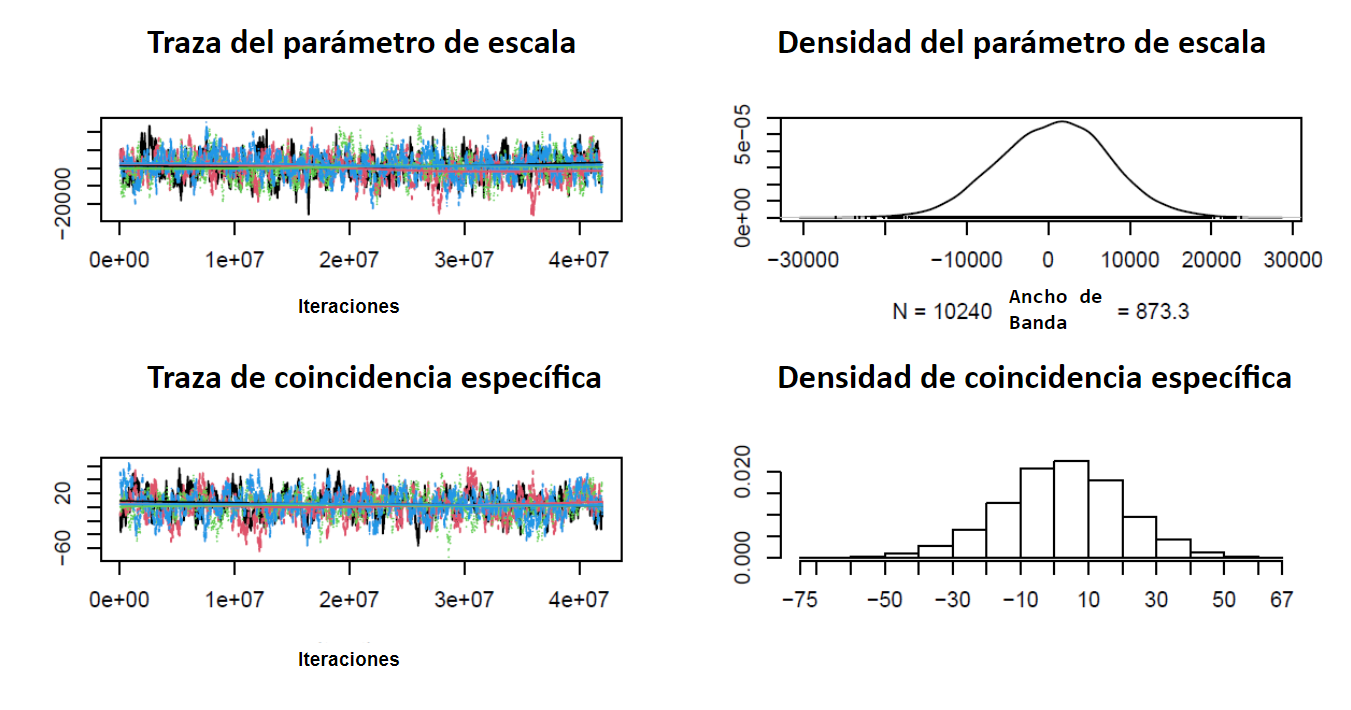
\includegraphics[width=1\textwidth]{Tesis/Figures/mcmc_specific2.PNG}
\caption{Diagnósticos de Markov del modelo de Triángulos Estrellas Alternantes y coincidencia de género específico}
\end{figure}

Viendo las medidas de bondad de ajuste aparentemente se ve mejor el modelo de coincidencia de géneros en específico al menos para la estadística de distancia geodésica. De forma interesante la distribución del grado de los nodos es mayor para el modelo de coincidencia de géneros en específico que para el de coincidencia de géneros en general. Una interpretación es que la coincidencia de género en específico genera comunidades de nodos más interconectados entre sí en donde se tiene grupos más conectados. Más información de estos modelos y sus características se pueden encontrar corriendo el código anexado y disponible en el \textit{github} del anexo.





\begin{figure}[!ht]
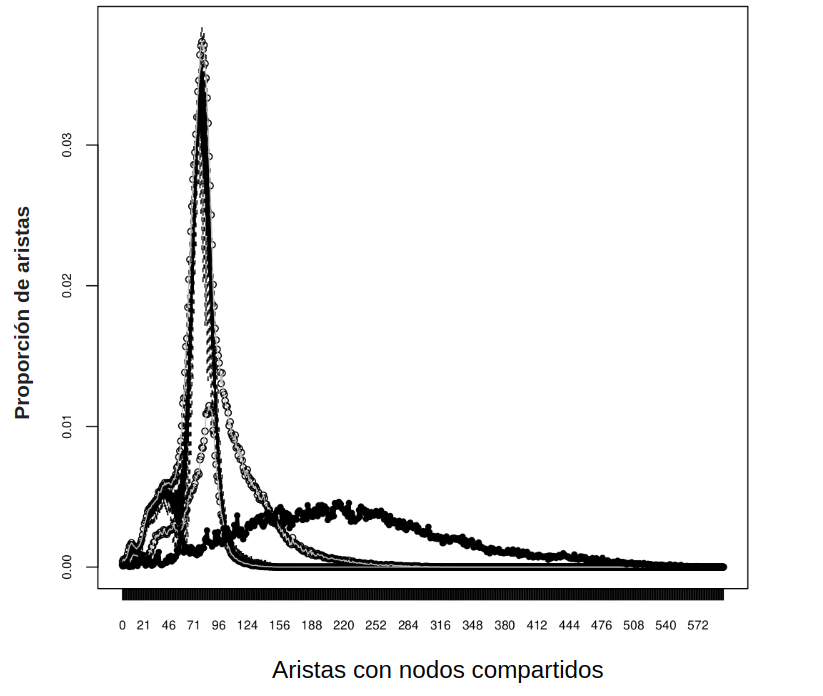
\includegraphics[width=.5\textwidth]{Tesis/Figures/gof_2_aristas_compartidas.png}
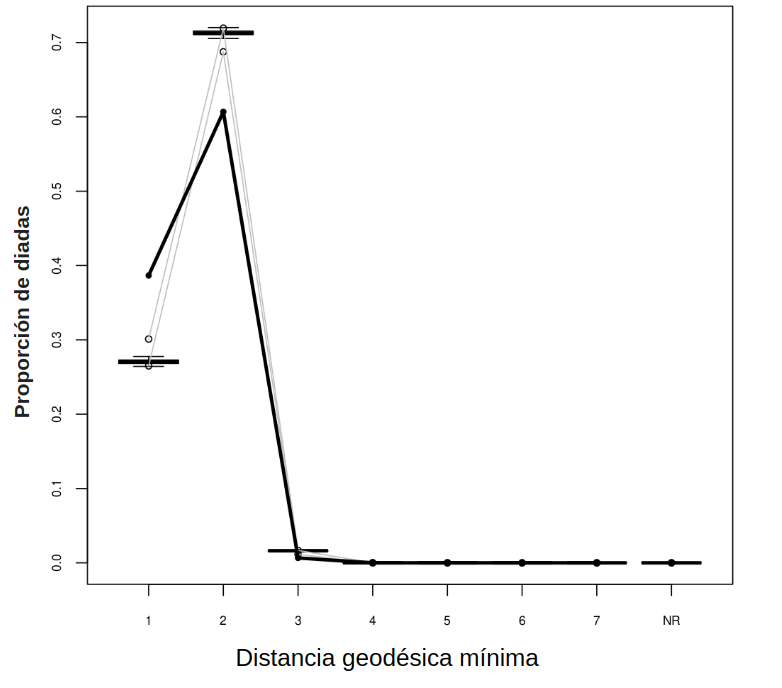
\includegraphics[width=.5\textwidth]{Tesis/Figures/gof_2_distancia.png}
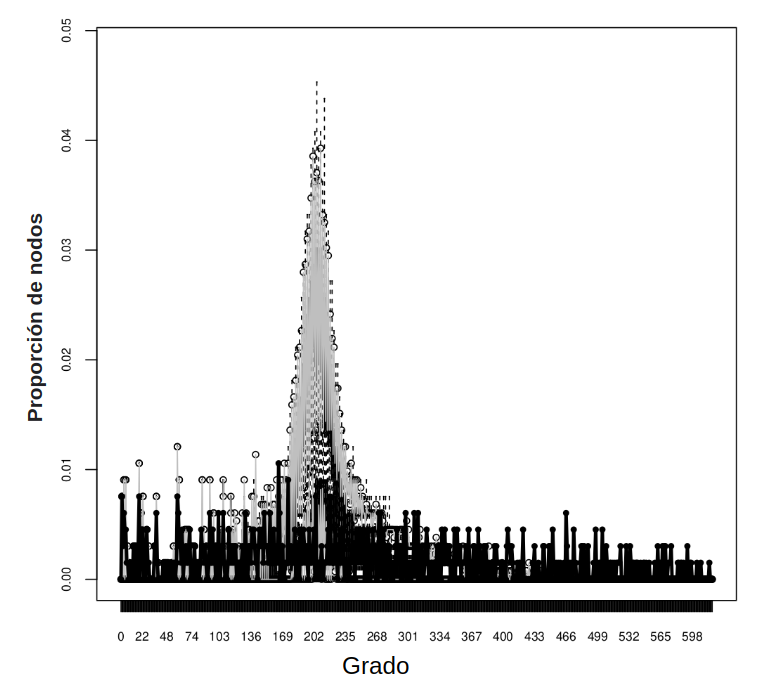
\includegraphics[width=.5\textwidth]{Tesis/Figures/gof_2_grado.png}
\caption{Medidas de bondad de ajuste del modelo de aristas, Triángulos Estrellas Alternantes  y coincidencia de género general}
\end{figure}


\begin{figure}[!ht]
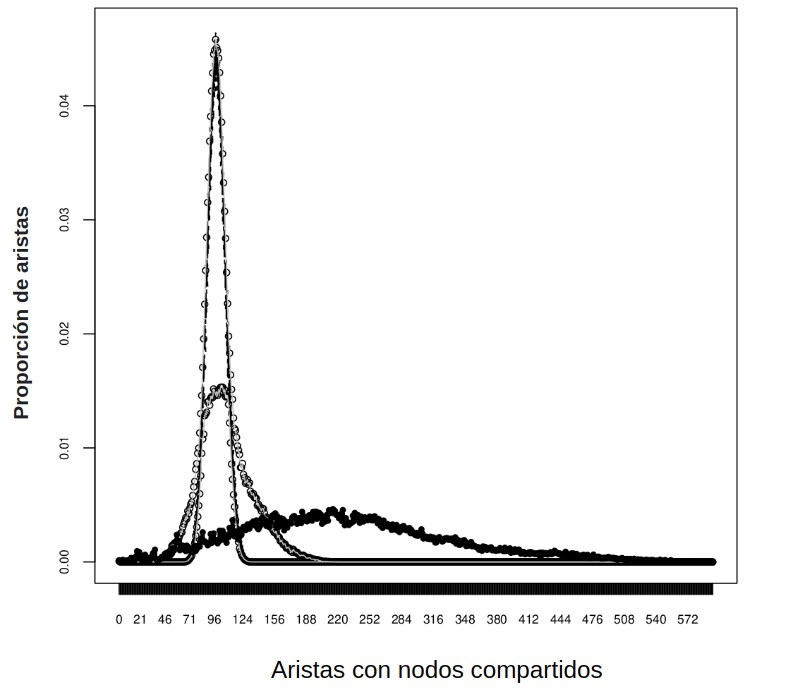
\includegraphics[width=.5\textwidth]{Tesis/Figures/gof_3_aristas_nodos_compartidos.png}
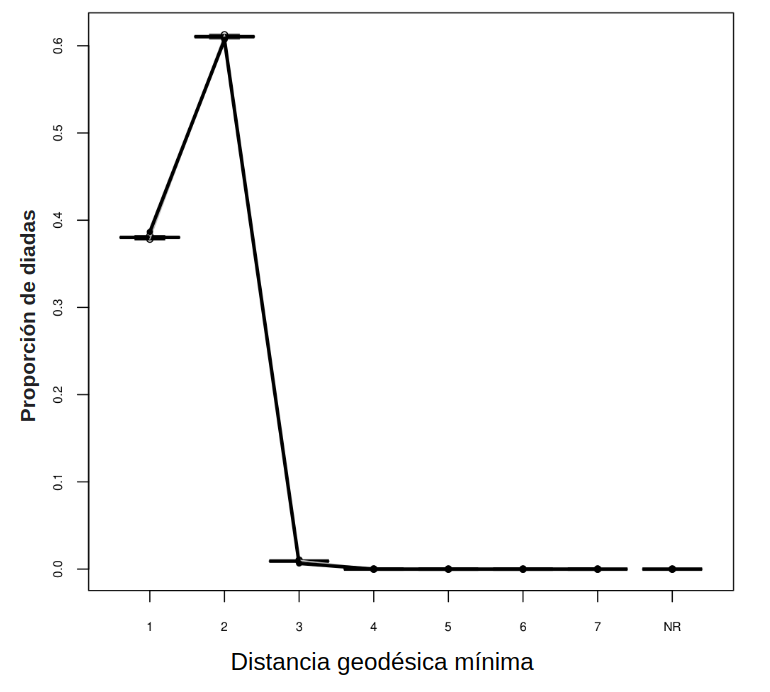
\includegraphics[width=.5\textwidth]{Tesis/Figures/gof_3_distancia.png}
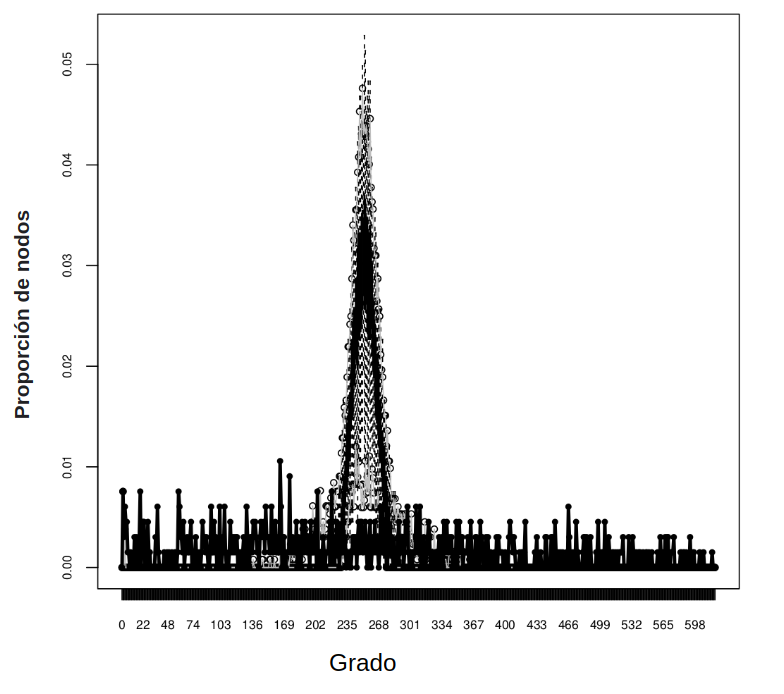
\includegraphics[width=.5\textwidth]{Tesis/Figures/gof_3_grado.png}
\caption{Medidas de bondad de ajuste del modelo de aristas, Triángulos Estrellas Alternantes y coincidencia de género específico}
\end{figure}